\documentclass[]{elsarticle}
\setlength{\marginparwidth}{0.5in}
\usepackage{amsmath,amssymb,amsthm,mathtools,bbm,booktabs,array,tikz,pifont,comment,graphicx}
\input FJHDef.tex

%Requires ApproxUnivariate.tex, univariate_integration.tex, foolbwquadexample.eps 

\DeclareMathOperator{\Var}{Var}
\DeclareMathOperator{\INT}{INT}
\DeclareMathOperator{\APP}{APP}
\DeclareMathOperator{\lin}{lin}
\DeclareMathOperator{\up}{up}
\DeclareMathOperator{\lo}{lo}
\DeclareMathOperator{\fix}{non}
\DeclareMathOperator{\err}{err}
\DeclareMathOperator{\maxcost}{maxcost}
\DeclareMathOperator{\mincost}{mincost}
\newcommand{\herr}{\widehat{\err}}

\newtheorem{theorem}{Theorem}
\newtheorem{prop}[theorem]{Proposition}
\newtheorem{lem}{Lemma}
\newtheorem{cor}{Corollary}
\theoremstyle{definition}
\newtheorem{algo}{Algorithm}
\newtheorem{condit}{Condition}
%\newtheorem{assump}{Assumption}
\theoremstyle{remark}
\newtheorem{rem}{Remark}
\newcommand{\Fnorm}[1]{\abs{#1}_{\cf}}
\newcommand{\Ftnorm}[1]{\abs{#1}_{\tcf}}
\newcommand{\Gnorm}[1]{\norm[\cg]{#1}}
\newcommand{\flin}{f_{\text{\rm{lin}}}}

\journal{Journal of Complexity}

\begin{document}

\begin{frontmatter}

\title{The Complexity of Deterministic Guaranteed Adaptive Automatic Algorithms:  Cones, Not Balls}
\author{Nicholas Clancy}
\author{Yuhan Ding}
\author{Caleb Hamilton}
\author{Fred J. Hickernell}
\author{Yizhi Zhang}
\address{Room E1-208, Department of Applied Mathematics, Illinois Institute of Technology,\\ 10 W.\ 32$^{\text{nd}}$ St., Chicago, IL 60616}
\begin{abstract} Automatic numerical algorithms are widely used in practice.  An algorithm that is automatic attempts to provide an approximate solution that differs from the true solution by no more than a user-specified error tolerance, $\varepsilon$. Furthermore, the computational effort required is typically determined adaptively by the algorithm based on function data, e.g., function values.  Ideally, the computational cost should match the difficulty of the problem.  Unfortunately, most automatic algorithms lack \emph{rigorous guarantees}, i.e., sufficient conditions on the input function that ensure the success of the algorithm. 

This article establishes a framework for automatic, adaptive algorithms that do have rigorous guarantees. Sufficient conditions for success and upper bounds on the computational cost are provided in Theorems \ref{TwoStageDetermThm} and \ref{MultiStageThm}.  Lower bounds on the complexity of the problem are given in Theorem \ref{complowbd} and conditions are given under which the proposed algorithms attain those lower bounds in Corollary \ref{optimcor}. These general theorems are illustrated with automatic algorithms for univariate numerical integration and function recovery.  Both algorithms use linear splines to approximate the input function.  

The key idea behind these automatic algorithms is that the error analysis should be done for \emph{cones} of input functions rather than balls. The existing literature contains certain negative results about the usefulness and reliability of automatic algorithms.  The theory presented does not share the assumptions on which those negative results are based, and so they are irrelevant.
\end{abstract}

\begin{keyword}
adaptive \sep automatic \sep cones \sep function recovery \sep integration \sep quadrature
%% keywords here, in the form: keyword \sep keyword

\MSC[2010] 65D05 \sep 65D30 \sep 65G20
%% MSC codes here, in the form: \MSC code \sep code
%% or \MSC[2008] code \sep code (2000 is the default)

\end{keyword}
\end{frontmatter}

\section{Introduction}

Automatic algorithms conveniently determine the computational effort required to obtain an approximate answer that is within a user-supplied error tolerance, $\varepsilon$, of the true answer.  Unfortunately, existing guaranteed automatic algorithms are typically not adaptive, meaning that the computational cost does not depend on the function values sampled by the algorithm.  On the other hand, adaptive automatic algorithms are typically not guaranteed to provide answers satisfying the error tolerance.  This article provides a way of constructing automatic algorithms that are both guaranteed and adaptive.

\subsection{Automatic Algorithms for Balls of Input Functions}
Let $\cf$ be a linear space of input functions with semi-norm $\Fnorm{\cdot}$, $\cg$ be a linear space of outputs with norm $\norm[\cg]{\cdot}$, and $S:\cf \to \cg$ be a \emph{solution operator}.  Suppose that one has a sequence of algorithms, $\{A_n\}_{n \in \ci}$, indexed by the computational cost $n$, where $\ci \subseteq \natzero$, and that these algorithms satisfy some known error bound:
\begin{subequations} \label{algoerr}
\begin{equation} \label{traditionerra}
\norm[\cg]{S(f)-A_n(f)} \le h(n) \Fnorm{f},
\end{equation}
where $h:\ci \to [0,\infty)$ is non-increasing. It is necessary for $A_n$ to be exact if the semi-norm of the input function vanishes, i.e., $S(f)=A_n(f)$ if $\Fnorm{f}=0$.   Define the (non-increasing) inverse of $h$ as 
\begin{equation} \label{hinvdef}
h^{-1}(\varepsilon) = \min \{n \in \ci : h(n) \le \varepsilon\}, \qquad \varepsilon > 0.
\end{equation}
\end{subequations}
Error bound \eqref{traditionerra} allows one to construct an automatic, but non-adaptive algorithm that is guaranteed for input functions in a prescribed $\cf$-ball.

\begin{algo} \label{nonadaptalgo} {\bf (Automatic, Non-Adaptive).} Let $\{A_n\}_{n \in \naturals}$ be defined as above, and let $\sigma$ be a fixed positive number.  Given  $\varepsilon$, a positive error tolerance, compute the computational cost needed to satisfy the error tolerance: $n=h^{-1}(\varepsilon/\sigma)$.
Then return $A_n(f)$ as the answer.
\end{algo}

\begin{theorem}  \label{NonAdaptDetermThm}  For $\cf$, $\Fnorm{\cdot}$, $\cg$, $\Gnorm{\cdot}$, $S$, as described above and under the assumptions of Algorithm \ref{nonadaptalgo}, if $f$ lies in the {\em ball} 
\begin{equation} 
\cb_\sigma=\{ f \in \cf : \Fnorm{f} \le \sigma\}, \label{balldef}
\end{equation}
then the answer provided by Algorithm \ref{nonadaptalgo} must satisfy the error tolerance, i.e., $\norm[\cg]{S(f)-A_n(f)} \le \varepsilon$.
\end{theorem}

While Algorithm \ref{nonadaptalgo} is guaranteed to return an answer with the desired accuracy by Theorem \ref{NonAdaptDetermThm}, this algorithm has drawbacks.  If this algorithm works for $f \in \cf$, it may not work for $cf \in \cf$, where $c$ is some constant, because $cf$ may fall outside the ball $\cb_\sigma$.  Moreover, although error bound \eqref{traditionerra} depends on $\Fnorm{f}$, the computational cost of Algorithm \ref{nonadaptalgo} does not depend on $\Fnorm{f}$.  The cost is the same whether $\Fnorm{f}=\sigma$ or $\Fnorm{f}$ is much smaller than $\sigma$.  This is because Algorithm \ref{nonadaptalgo} makes no use of the function values sampled to estimate $\Fnorm{f}$.

\subsection{Adaptive Automatic Algorithms for Cones of Input Functions} \label{adapintrosec}

Adaptive automatic algorithms are common in numerical software packages.  Examples include  MATLAB's {\tt quad} and {\tt integral} \cite{MAT8.1}, the quadrature algorithms in the NAG Library \cite{NAG23}, and the MATLAB Chebfun toolbox \cite{TrefEtal12}.  While these adaptive algorithms work well in practice for many cases, they do not have rigorous guarantees of success. The methods used to determine the computational cost are heuristics or either asymptotic error estimates that do not necessarily hold for finite sample sizes.

In this article we derive guaranteed adaptive automatic algorithms by using function data to construct a \emph{rigorous} upper bound on the semi-norm $\Fnorm{f}$ that appears in \eqref{traditionerra}.  The details are presented in Section \ref{genthmsec}, but we summarize the argument here.  The key idea is to consider functions lying in a \emph{cone}, not a ball.  A cone is a set with the property that any positive multiple of an element in the set is also in the set.

Let $\Ftnorm{\cdot}$ be some weaker semi-norm than $\Fnorm{\cdot}$, i.e., there exists a positive constant $\tau_{\min}$ for which 
\begin{equation} \label{Fspacecondstrong}
\tau_{\min} \Ftnorm{f} \le \Fnorm{f} \qquad \forall f \in \cf.
\end{equation}
The $\tcf$-semi-norm should be weak enough that $\Ftnorm{f}$ can be estimated using function data as accurately as needed with a computational cost depending on $\Fnorm{f}$.  To assure that $\Ftnorm{f}$ can be estimated with reasonable cost, $f$ is assumed to lie in the cone 
\begin{equation} \label{conedef}
\cc_{\tau}=\{f \in \cf : \Fnorm{f} \le \tau \Ftnorm{f} \}.
\end{equation}
Note that functions in this cone may have arbitrarily large $\cf$- and $\tcf$-semi-norms.  Since the stronger norm is now bounded above by a constant times the weaker norm, it is possible to construct reliable data-based upper bounds for $\Ftnorm{f}$ and $\Fnorm{f}$.  This latter upper bound allows one to determine the computational cost needed to estimate $S(f)$ via error bound \eqref{traditionerra}.

An explicit application of these ideas to the problem of evaluating $\int_0^1 f(x) \, \dif x$ is provided in Section \ref{integsec}.  There $\cf$ is the set of all continuous functions whose first derivatives have finite (total) variation, $\Fnorm{f}=\Var(f')$, and $\Ftnorm{f}=\norm[1]{f'}$.  The algorithm used is the composite equal-width trapezoidal rule.  The cost of the guaranteed adaptive automatic algorithm is no greater than $4+ \tau + \sqrt{\tau \Var(f')/(4\varepsilon)}$ (Theorem \ref{multistageintegthm}), where $\Var(f')$ is unknown a priori. Here $\tau$ represents is related to the minimum sample size, and $1/\tau$ represents a length scale of for possible spikes that one wishes to integrate accurately.

\subsection{Scope and Outline of this Article} 
There are limited theoretical results providing conditions under which adaption is useful.  Novak \cite{Nov96a} shows the advantage of adaption in for some problems in the average case and randomized settings.  Plaskota and Wasilkowski \cite{PlaWas05a,PlaEtal08a} demonstrate the advantage of adaption for integrating or approximating functions with singularities. By contrast, here we consider the deterministic setting, and we are not concerned with functions with singularities.

This article starts with the general setting and then moves to two concrete cases.  Section \ref{probdefsec} defines the problems to be solved and introduces our notation.  Sections \ref{genthmsec} and \ref{LowBoundSec} describe the automatic algorithms in detail and provides proofs of their success for cones of input functions.  Although the long term goal of this research is to construct good locally adaptive algorithms, where the sampling density varies according to the function data, here we present only globally adaptive algorithms, where the sampling density is constant, but the number of samples is determined adaptively.  Section \ref{integsec} illustrates the general results in Sections \ref{genthmsec} and \ref{LowBoundSec} for the univariate integration problem.  Section \ref{approxsec}  presents analogous results for function approximation.  Common concerns about automatic and adaptive algorithms are answered in Section \ref{overcomesec}. The article ends with several suggestions for future work.

\section{General Problem Definition} \label{probdefsec}

\subsection{Problems and Algorithms} The function approximation, integration, or other problem to be solved is defined by a solution operator $S:\cf \to \cg$, where $(\cf,\Fnorm{\cdot})$ is a semi-normed linear space of possible input functions defined on $\cx$, and $(\cg,\norm[\cg]{\cdot})$ is some other normed linear space of possible outputs or solutions. The solution operator is assumed to be positively homogeneous, i.e., 
\[
S(cf) = cS(f) \qquad \forall c\ge 0.
\]
Examples include the following:
\begin{align*}
\text{Integration:} \quad & S(f) = \int_{\cx} f(\vx) \, w(\vx) \, \dif \vx, \quad w \text{ is fixed,}\\
\text{Function Recovery:} \quad & S(f) = f, \\
\text{Poisson's Equation:} \quad & S(f) = u, \quad \text{where } \begin{array}{c} -\Delta u(\vx) = f(\vx), \ \vx \in \cx, \\ u(\vx)=0 \ \forall \vx \in \partial \cx, \text{ and}\end{array} \\
\text{Optimization:} \quad & S(f) = \min_{\vx \in \cx} f(\vx).
\end{align*}
The first three examples above are linear problems, but the last example is a nonlinear problem, which nevertheless is positively homogeneous.

An automatic algorithm $A:\cf\times(0,\infty) \to \cg$ takes as inputs a function, $f$, and an error tolerance, $\varepsilon$.  Our goal is to find efficient $A$ for which $\norm[\cg]{S(f)-A(f,\varepsilon)}\le \varepsilon$.  Algorithm \ref{nonadaptalgo} is one non-adaptive example that is successful for functions in balls.

Following the definition of algorithms described in \cite[Section 3.2]{TraWasWoz88}, the algorithm takes the form of some function of data derived from the input function:
\begin{equation}
\label{algoform}
A(f,\varepsilon) =  \phi(\vL(f)), \quad \vL(f) = \left(L_1(f), \ldots, L_m(f)\right) \qquad \forall f \in \cf.
\end{equation}
Here the $L_i \in \Lambda$ are real-valued homogeneous functions defined on $\cf$:
\begin{equation}
\label{dataassump}
L(cf) = cL(f) \qquad \forall f \in \cf, \ c \in \reals, \ L \in \Lambda.
\end{equation}
One popular choice for $\Lambda$ is the set of all function values, $\Lambda^{\std}$, i.e., $L_i(f) = f(\vx_i)$ for some $\vx_i \in \cx$.  Another common choice is the set of all bounded linear functionals, $\Lambda^{\lin}$.  In general, $m$ may depend on $f$, and $\varepsilon$, and the choice of $L_i$ may depend on $L_1(f), \ldots, L_{i-1}(f)$.  The set of all such algorithms is denoted $\ca(\cf,\cg,S,\Lambda)$. In this article, all algorithms are assumed to be deterministic.  There is no random element.

In most cases the algorithms we consider are designed for input functions lying in some proper subset of $\cf$, such as a ball or a cone.  Algorithms that know that the input function comes from $\cn \subseteq \cf$ are said to lie in $\ca(\cn,\cg,S,\Lambda)$. For example, Algorithm \ref{nonadaptalgo} lies $\ca(\cb_{\sigma},\cg,S,\Lambda)$.  

\subsection{Costs of Algorithms} \label{AlgoCostsec}

The cost of a possibly adaptive algorithm, $A$, depends on the function and the error tolerance: 
\[
\cost(A,f,\varepsilon) = \$(\vL) = \$(L_1) + \cdots +\$(L_m) \in \natzero,
\]
where $\$:\Lambda \to \naturals$, and $\$(L)$ is the cost of acquiring the datum $L(f)$. The cost of $L$ may be the same for all $L \in \Lambda$, e.g, $\$(L)=1$.  Alternatively, the cost might vary with the choice of $L$.  For example, if $f$ is a function of the infinite sequence of real numbers, $(x_1, x_2, \ldots)$, the cost of evaluating the function with arbitrary values of the first $d$ coordinates, $L(f)=f(x_1, \ldots, x_d, 0, 0, \ldots)$, might be $d$.  This cost model has been used by \cite{HicMGRitNiu09a,KuoEtal10a,NiuHic09a,NiuHic09b,PlaWas11a} for integration problems and \cite{Was13a,WasWoz11a,WasWoz11b} for function approximation problems.  If an algorithm does not require any function data, then its cost is zero.

Although the cost of an adaptive algorithm varies with $f$, we hope that it does not vary wildly for different input functions with the same $\cf$-semi-norm. We define the \emph{maximum} and \emph{minimum} costs of the algorithm $A\in \ca(\cn,\cg,S,\Lambda)$ relative to $\cb_{\sigma}$, the $\cf$-semi-norm ball, as follows:
\begin{gather*}
\maxcost(A,\cn,\varepsilon,\cb_s)
= \sup \{ \cost(A,f,\varepsilon) : f \in \cn \cap \cb_{s} \}, \\ \mincost(A,\cn,\varepsilon,\cb_s)
= \inf \left \{ \cost(A,f,\varepsilon) : f \in \cn\setminus \bigcup_{s'<s}\cb_{s'} \right\} .
\end{gather*}
We stress that $A$ knows that $f \in \cn$ but does not necessarily know $\Fnorm{f}$.  An algorithm is said to have \emph{$\cb_{\sigma}$-stable computational cost} if 
\begin{equation}\label{coststabledef}
\sup_{\varepsilon, s > 0} \frac{\maxcost(A,\cn,\varepsilon,\cb_s)}{\max(1,\mincost(A,\cn,\varepsilon, \cb_s))} < \infty.
\end{equation} 
Analogous definitions of maximum and minimum cost and stability of computational cost can be made in terms of $\tcf$-semi-norm balls.

The complexity of a problem is defined as the maximum cost of the cheapest algorithm that always satisfies the error tolerance:
\begin{multline} \label{complexdef}
\comp(\varepsilon,\ca(\cn,\cg,S,\Lambda),\cb_s) \\
 = \inf\left\{\maxcost(A,\cn,\varepsilon,\cb_s) : A \in \ca(\cn,\cg,S,\Lambda), \right. \\
 \left . \norm[\cg]{S(f)-A(f,\varepsilon)} \le \varepsilon \ \ \forall \varepsilon \ge 0 \right \} \in \natzero.
\end{multline}
Here the infimum of an empty set is defined to be $\infty$.  An adaptive automatic algorithm is \emph{optimal} if its cost tracks that of the best possible possible algorithm, i.e.,
\begin{equation} \label{nearoptdef}
\sup_{\varepsilon,\sigma > 0} \frac{\maxcost(A,\cn,\varepsilon,\cb_s)} {\max(1,\comp(\varepsilon,\ca(\cn,\cg,S,\Lambda),\cb_s))} <\infty.
\end{equation}

Algorithm \ref{nonadaptalgo} is an example of an algorithm that fits the framework described above.  It is defined for input functions lying in the ball $\cb_{\sigma}$.  It is automatic, though not adaptive, and takes as its inputs a function, $f$, and an error tolerance, $\varepsilon$.  It has a cost that depends only on $\varepsilon/\sigma$, and not on the particulars of $f$:
\begin{equation} \label{nonadaptalgocost}
\maxcost(A,\cb_{\sigma},\varepsilon,\cb_{s}) = \mincost(A,\cb_{\sigma},\varepsilon,\cb_{s}) = \cost(A,f,\varepsilon) = h^{-1}(\varepsilon/\sigma).
\end{equation}
The optimality of Algorithm \ref{nonadaptalgo} depends on whether $h$ satisfies condition \eqref{ghcond} below.

\subsection{Non-Automatic Algorithms}

Algorithm \ref{nonadaptalgo} is built using a sequence of non-automatic, fixed cost algorithms, $\{A_n\}_{n \in \ci}$, indexed by their cost and defined for all $f \in \cf$.  The set of non-automatic algorithms is denoted $\ca_{\fix}(\cf,\cg,S,\Lambda)$.  These are algorithms for which neither the choice of the $L_i$ nor the number of function data depend on the input function.  Furthermore, such non-automatic algorithms have no dependence on $\varepsilon$, so we will typically write $A_n(f)$ rather than $A_n(f,\varepsilon)$ for convenience sake.  Any non-automatic algorithm, $A_n \in \ca_{\fix}(\cf,\cg,S,\Lambda)$ is assumed to be satisfy the following positive homogeneity properties:
\begin{equation}
\label{algoscale}
\vL(cf) = c \vL(f), \ \
\phi(c\vy) = c\phi(\vy), \ \ A_n(cf) = cA_n(f) \quad \forall c \ge 0, \ \vy \in \reals^m.
\end{equation}
These conditions make the error of these algorithms homogeneous, resulting in error bounds involving a non-increasing $h$ as described in \eqref{algoerr}.

The adaptive, automatic algorithms constructed in the next section use sequences of non-automatic algorithms indexed by their cost that converge to the true answer as the cost increases:
\begin{subequations} \label{algseqerrcond}
\begin{equation} \label{algseqdef}
\{A_n\}_{n \in \ci}, \quad A_n  \in \ca_{\fix}(\cf,\cg,S,\Lambda), \quad \cost(A_n) = n, \quad
\inf_{n \in \ci} h(n) = 0.  
\end{equation}
Here in this article the positive integer-valued index set, $\ci=\{n_1, n_2, \ldots\} \subseteq \natzero$, with $n_i < n_{i+1}$ is assumed to satisfy 
\begin{equation} \label{Inobiggap}
\sup_i \frac{n_{i+1}}{n_i} \le \rho <\infty.
\end{equation}
Note that the definition of $h^{-1}$ in \eqref{hinvdef} implies that
\begin{equation}
h(n)\le\varepsilon \implies n \ge h^{-1}(\varepsilon), \qquad  h(n) > \varepsilon \implies  n < h^{-1}(\varepsilon).
\end{equation}
Finally, in this article we consider sequences of algorithms for which $h$ satisfies
\begin{equation} \label{hinvonetwocond}
\sup_{\epsilon > 0} \frac{h^{-1}(\varepsilon)}{h^{-1}(2\varepsilon)} < \infty.
\end{equation}
\end{subequations}
This means that $h(n)$ may decay polynomially in $n^{-1}$ or faster as $n$ tends to infinity.

\section{General Algorithms and Upper Bounds on the Complexity} \label{genthmsec}

This section provides rather general theorems about the complexity of automatic algorithms.  In some sense, these theorems are a road map because their assumptions are non-trivial and require effort to verify for specific problems of interest.  On the other hand, the assumptions are reasonable as is demonstrated by the concrete examples in Sections \ref{integsec} and \ref{approxsec}.  

\subsection{Bounding the $\tcf$-Semi-Norm} \label{Galgosec}

As mentioned in Section \ref{adapintrosec} adaptive automatic algorithms require reliable upper bounds on $\Ftnorm{f}$ for all $f$ in the cone $\cc_{\tau}$. These can be obtained using any non-automatic algorithm $\tF_n \in \ca_{\fix}(\cf,\reals_+,\Ftnorm{\cdot},\Lambda)$ for approximating $\Ftnorm{f}$ for $f \in \cf$ and having cost $n$, provided that one has explicit upper bounds on the errors of these algorithms.  This means that there exist non-negative valued, non-increasing functions $h_{\pm}$ such that
\begin{equation} \label{Gerrbds}
-h_{-}(n)\Fnorm{f} \le \Ftnorm{f}- \tF_n(f) \le h_{+}(n) \Fnorm{f}, \qquad \forall f \in \cf.
\end{equation}
This implies that $\tF_n(f)=\Ftnorm{f}$ for all $f \in \cf$ with vanishing $\cf$-semi-norm.  Applying the two bounds for the $\cf$- and $\tcf$-semi-norms in \eqref{Fspacecondstrong} and \eqref{conedef} and rearranging the above error bound implies that 
\begin{align*} 
\tF_n(f) &\le \Ftnorm{f} + h_{-}(n)\Fnorm{f} \le \begin{cases} [1+ \tau h_{-}(n)]\Ftnorm{f} \\
\displaystyle \left [\frac{1}{\tau_{\min}}+h_{-}(n) \right]\Fnorm{f} 
\end{cases} \qquad \forall f \in \cc_{\tau},\\
\tF_n(f) &\ge \Ftnorm{f} - h_{+}(n)\Fnorm{f} \ge \begin{cases} [1 - \tau h_{+}(n)]\Ftnorm{f} \\
\displaystyle \left [\frac{1}{\tau}-h_{+}(n) \right]\Fnorm{f} 
\end{cases} \qquad \forall f \in \cc_{\tau}.
\end{align*}

\begin{lem} \label{Gnormlem} Any non-automatic algorithm $\tF_n \in \ca_{\fix}(\cf,\reals_+,\Ftnorm{\cdot},\Lambda)$ with cost $n=\cost(\tF_n)$ and two sided error bounds as in \eqref{Gerrbds} yields an approximation to the $\tcf$-semi-norm of functions in the cone $\cc_{\tau}$ with the following upper and lower error bounds:
\begin{equation} \label{twosidedGineq}
 \frac{\Fnorm{f}}{\tau \fC_n}  \le \frac{\Ftnorm{f}}{\fC_n}  \le \tF_n(f) \le  \begin{cases} \tfc_n \Ftnorm{f} \\[1ex]
\displaystyle \frac{\fc_n \Fnorm{f} }{\tau_{\min}}
\end{cases} \qquad \forall f \in \cc_{\tau},
\end{equation}
where the $\fc_n$, $\tfc_n$, and $\fC_n$ are defined as follows:
\begin{gather} \label{normdeflate}
\tfc_n :=1 + \tau h_{ -}(n)  \ge \fc_n :=1 + \tau_{\min} h_{ -}(n)  \ge 1, \\
\label{norminflate}
\fC_n :=\frac{1}{1 - \tau h_{ +}(n)} \ge 1, \qquad \text{assuming } h_{ +}(n) < 1/\tau.
\end{gather}
\end{lem}

\subsection{Two-Stage Automatic Algorithms} \label{twostagesec}

Computing an approximate solution to the problem $S: \cc_{\tau} \to \cg$, e.g., integration or function approximation also depends on a sequence of non-automatic algorithms, $\{A_n\}_{n \in \ci}$, satisfying \eqref{algoerr} and \eqref{algseqerrcond}.  One may then use the upper bound in Lemma \eqref{Gnormlem} to construct a data-generated upper bound on the error:
\begin{equation} \label{Anerrbound}
\norm[\cg]{S(f) -  A_n(f)} \le h(n)\Fnorm{f} \le \tau  \fC_n h(n)\tF_n(f) \qquad \forall f \in \cc_{\tau}.
\end{equation}

\begin{algo} \label{twostagedetalgo} {\bf (Adaptive, Automatic, Two-Stage).} Let $\tau$ be a fixed positive number, and let $\tF_{n_{\tF}}$ be an algorithm as described in Lemma \ref{Gnormlem} with cost $n_{\tF}$ satisfying $h_{+}(n_{\tF}) < 1/\tau$.
Moreover, let  $\{A_n\}_{n \in \ci}$ be a sequence of algorithms as described in \eqref{algoerr} and \eqref{algseqerrcond}.  Given  a positive error tolerance, $\varepsilon$, and  an input function $f$, do the following:

\begin{description} 

\item[Step 1.\ Bound {$\Fnorm{f}$}.] First compute $\tF_{n_{\tF}}(f)$.  Define the inflation factor $\fC=\fC_{n_{\tF}}$ according to \eqref{norminflate}.
Then $\tau \fC \tF_{n_{\tF}}(f)$ provides a reliable upper bound on $\Fnorm{f}$.  

\item [Step 2.\ Estimate {$S(f)$}.] Choose the sample size need to approximate $S(f)$, namely, $n_A=h^{-1}(\varepsilon/(\tau\fC \tF_{n_{\tF}}(f)))$.  Finally, return $A_{n_A}(f)$ as the approximation to $S(f)$ at a total cost of $n_{\tF}+n_A$. 
\end{description}
\end{algo}

The bounds in Lemma \ref{Gnormlem} involving $\tF_n$ imply bounds on the cost in the algorithm above.  Since $h^{-1}$ is a non-increasing function, it follows that for all $f \in \cc_{\tau}$
\begin{equation*}
h^{-1}\left(\frac{\varepsilon}{\Fnorm{f}}\right) \le  h^{-1}\left(\frac{\varepsilon}{\tau\Ftnorm{f}}\right)  \le h^{-1}\left(\frac{\varepsilon}{\tau \fC \tF_{n_{\tF}}(f)}\right) \le 
\begin{cases} \displaystyle  h^{-1}\left(\frac{\varepsilon}{\tau \fC \tfc \Ftnorm{f}}\right) \\[2ex]
\displaystyle  h^{-1}\left(\frac{\tau_{\min} \varepsilon}{\tau \fC \fc \Fnorm{f}}\right)\end{cases}.
\end{equation*}

\begin{theorem}  \label{TwoStageDetermThm}  Let $\cf$, $\Fnorm{\cdot}$, $\Ftnorm{\cdot}$, $\cg$, $\Gnorm{\cdot}$, and $S$ be as described above.  Under the assumptions of Algorithm  \ref{twostagedetalgo}, let $\fc=\fc_{n_{\tF}}$ be defined as in \eqref{normdeflate}.
Let $\cc_\tau$ be the cone of functions defined in \eqref{conedef} whose $\cf$-semi-norms are no larger than $\tau$ times their $\tcf$-semi-norms.  Then it follows that Algorithm \ref{twostagedetalgo}, which lies in $\ca(\cc_{\tau},\cg,S,\Lambda)$, is successful,  i.e.,  $\norm[\cg]{S(f)-A(f,\varepsilon)} \le \varepsilon$ for all $f \in \cc_\tau$.  Moreover, the cost of this algorithm is bounded above and below in terms of the unknown $\tcf$- and $\cf$-semi-norms of any input function in $\cc_{\tau}$ as follows:
\begin{subequations}  \label{auto2stagedetcost}
\begin{gather}
n_{\tF}+ h^{-1}\left(\frac{\varepsilon}{\tau \Ftnorm{f}} \right) \le 
\cost(A,f,\varepsilon)
\le n_{\tF}+ h^{-1}\left(\frac{\varepsilon}{\tau \fC\tfc\Ftnorm{f}}\right), \\
n_{\tF}+ h^{-1}\left(\frac{\varepsilon}{\Fnorm{f}} \right) \le \cost(A,f,\varepsilon)
\le n_{\tF}+h^{-1}\left(\frac{\tau_{\min}\varepsilon}{\tau \fC\fc\Fnorm{f}}\right).
\end{gather}
\end{subequations}
Since $h$ satisfies \eqref{algseqerrcond}, then this algorithm is computationally stable in the sense that the maximum cost is no greater than some constant times the minimum cost, both for $\tcf$-balls and $\cf$-balls.
\end{theorem}

\begin{proof} The choice of $n_A$ in Algorithm \ref{twostagedetalgo} ensures that the right hand side of \eqref{Anerrbound} is no greater than the error tolerance, so the algorithm is successful, as claimed in the theorem.  The argument preceding the statement of this theorem establishes the maximum and minimum cost bounds in \eqref{auto2stagedetcost}. 
\end{proof}

There are a several points to note about this result.

\begin{rem} Two main conditions must be checked for this theorem to hold.
\begin{enumerate}
\renewcommand{\labelenumi}{\roman{enumi}.}
\item There must be an algorithm, $\tF_n$, that approximates the weaker semi-norm,  $\Ftnorm{\cdot}$, and its error bound, $h_{\pm}$, as defined in \eqref{Gerrbds} must be known explicitly, as described in Section \ref{Galgosec}.
\item There must be a  sequence of nonadaptive algorithms, $\{A_n\}_{n \in \ci}$, as described at the beginning of  Section \ref{twostagesec}, and the error function $h$, defined in \eqref{algoerr} must be known explicitly.  
\end{enumerate}
Sections \ref{integsec} and \ref{approxsec} provide concrete examples where these conditions are checked.
\end{rem}

\begin{rem} The maximum and minimum costs of Algorithm \ref{twostagedetalgo}, as given by \eqref{auto2stagedetcost}, depend on the $\cf$- and $\tcf$-semi-norms of the input function, $f$.  However, the values of these semi-norms are not inputs to the algorithm, but rather are bounded by the algorithm.  The number of samples used to obtain the approximation to $S(f)$ is adjusted adaptively based on these bounds.
\end{rem}

\begin{rem} Instead of choosing $\tau$ as an input parameter for Algorithm \ref{twostagedetalgo}, one may alternatively choose the inflation factor $\fC >1$.  This then implies that 
\begin{equation} \label{taufromnC}
\tau = \left(1 - \frac{1}{\fC}\right)\frac{1}{h_{+}(n_{\tF})},
\end{equation}
which is equivalent to \eqref{norminflate}.
\end{rem}

\begin{rem} \label{neccondrem} In some cases it is possible to find a lower bound on the $\cf$-norm of the input function.  This means that there exists an algorithm $F_n$ using the same function values as $\tF_n$, such that
\[
F_n(f) \le \Fnorm{f} \qquad \forall f \in \cf.
\]
When such an $F_n$ is known, Lemma \ref{Gnormlem} can be used to derive a necessary condition that $f$ is in the cone $\cc_\tau$:
\begin{align}
\nonumber
f \in \cc_\tau 
& \implies F_n(f) \le \Fnorm{f} \le \frac{\tau \tF_n(f)}{1-\tau h_+(n)}\\
& \implies \tau_{\min,n}:= \frac{F_n(f)}{\tF_n(f) + h_+(n) F_n(f)} \le \tau.
\label{neccondFn}
\end{align}
For Algorithm \ref{twostagedetalgo} the relevant value of $n$ is $n_{\tF}$, whereas for Algorithm \ref{multistagealgo} the relevant value of $n$ is $n_i$.
We stress that this is not a sufficient condition for $f$ to lie in $\cc_{\tau}$, so it is possible to get an incorrect answer from Algorithm \ref{twostagedetalgo} or \ref{multistagealgo} even if \eqref{neccondFn} is satisfied but $f \notin \cc_{\tau}$.  However, in light of this argument one might modify these algorithms by increasing $\tau$ to, say, $2 \tau_{\min,n}$ whenever  $\tau_{\min,n}$ rises above $\tau$. 
\end{rem}

\subsection{Automatic Algorithms Based on Embedded Algorithms $\{A_n\}_{n \in \ci}$}

Suppose that the sequence of nonadaptive algorithms, 
\[
\{A_n\}_{n \in \ci} = \{A_{n_1}, A_{n_2}, \ldots \}, 
\]
are \emph{embedded}, i.e., $A_{n_{i+1}}$ uses all of the data used by $A_{n_{i}}$ for $i=1, 2, \ldots$.  An example would be a sequence of composite trapezoidal rules for integration where the number of trapezoids is a power of two. Furthermore, suppose that the data used by $\tF_{n_{\tF}}$, the algorithm used to estimate the $\tcf$-semi-norm of $f$, is the same data used by $A_{n_1}$, and so $n_1=n_{\tF}$.  Then the total cost of Algorithm \ref{twostagedetalgo} can be reduced to simply $n_A$, as given in Step 2, instead of $n_{\tF}+n_A$.

Again suppose that $\{A_n\}_{n \in \ci}$, $A_n  \in \ca_{\fix}(\cf,\cg,S,\Lambda)$, consists of algorithms as described in \eqref{algoerr} and \eqref{algseqerrcond}, but some of which are embedded in others.  An example would be all possible composite trapezoidal rules for integration that use trapezoids of equal widths.   Moreover, suppose that there exists some fixed $r > 1$ such that for all $n \in \ci$, there exists a $\tn \in \ci$ with $n < \tn \le rn$, such that the data for $A_n$ is embedded in the data for $A_{\tn}$. One may think of $r$ as the minimum cost multiple that one must incur when moving to the next more costly algorithm. For trapezoidal rules, where the cost is the number of trapezoids plus one, one may take $\tn-1=2(n-1)$, so one may choose $r=2$.

Suppose also that there exists a sequence of algorithms for approximating the $\tcf$-semi-norm, $\{\tF_n\}_{n \in \ci}$, $\tF_n  \in \ca_{\fix}(\cf,\reals_+,\Ftnorm{\cdot},\Lambda)$, such that for each $n \in \ci$, $A_n$ and $\tF_n$ use exactly the same data.
Since $h_{\pm}$ are non-increasing functions, the quantities $\fC_{n}$ and $\fc_n$ do not increase as $n$ increases. These embedded algorithms suggest the following iterative algorithm.

\begin{algo} \label{multistagealgo}  Let the sequences of algorithms, $\{A_n\}_{n \in \ci}$ and  $\{\tF_n\}_{n \in \ci}$ be as described above.  Let $\tau$ be the positive cone constant. Set $i=1$, and $n_1 = \min\{ n \in \ci : h_+(n) < 1/\tau\}$. For any positive error tolerance $\varepsilon$ and any input function $f$, do the following:
\begin{description}

\item [Step 1. Estimate $\Ftnorm{f}$.] Compute $\tF_{n_i}(f)$ and $\fC_{n_i}$ as defined in \eqref{norminflate}.  

\item [Step 2. Check for Convergence.] Check whether $n_i$ is large enough to satisfy the error tolerance, i.e., 
\begin{equation} \label{multistageconv}
\tau \fC_{n_i} h(n_i)\tF_{n_i}(f) \le \varepsilon.
\end{equation}
If this is true, return $A_{n_i}(f)$ and terminate the algorithm.

\item[Step 3. Compute $n_{i+1}$.]  Otherwise, if \eqref{multistageconv} fails to hold, compute $\fc_{n_i}$ according to \eqref{normdeflate}, and choose $n_{i+1}$ as the smallest number exceeding $n_i$ and not less than $h^{-1}(\varepsilon \tfc_{n_i}/[\tau \tF_{n_i}(f)])$ such that $A_{n_{i}}$ is embedded in $A_{n_{i+1}}$. Increment $i$ by $1$, and return to Step 1.  

\end{description}  
\end{algo}

This iterative algorithm is guaranteed to converge also, and its cost can be bounded.  Define 
\begin{equation} \label{hhdef}
h_1(n) := \fC_n\tfc_n h(n) \ge h(n), \quad h_2(n) := \fC_n\fc_n h(n) \ge h(n) \qquad n \in \ci.
\end{equation}
and note that $h_1$ and $h_2$ are non-increasing functions.  Let $h_1^{-1}$ and $h_2^{-1}$ be defined analogously to $h^{-1}$ as in \eqref{hinvdef}.  These definitions imply that the quantity appearing on the left hand side of \eqref{multistageconv}, has the following upper and lower bounds based on \eqref{twosidedGineq} for $f \in \cc_{\tau}$:
\begin{subequations}\label{hh1h2bounds}
\begin{equation}
h(n)\Fnorm{f} \le \tau h(n)\Ftnorm{f} \le \tau \fC_{n} h(n)\tF_{n}(f) \le \begin{cases} \tau h_1(n) \Ftnorm{f} \\[1ex]
\displaystyle \frac{\tau h_2(n) \Fnorm{f} }{\tau_{\min}}
\end{cases} , \quad n \in \ci,
\end{equation}
\begin{multline}
h^{-1}\left(\frac{\varepsilon}{\Fnorm{f}}\right) \le h^{-1}\left(\frac{\varepsilon}{\tau \Ftnorm{f}}\right) \le \min\{n : \tau \fC_{n} h(n)\tF_{n}(f) \le \varepsilon\} \\
\le \begin{cases} \displaystyle h_1^{-1}\left(\frac{\varepsilon}{\tau \Ftnorm{f}} \right) \\[2ex]
\displaystyle h_2^{-1}\left(\frac{\tau_{\min}\varepsilon}{\tau \Fnorm{f}} \right)
\end{cases} , \qquad \varepsilon > 0.
\end{multline}
\end{subequations}
These inequalities may be used to prove the following theorem about Algorithm \ref{multistagealgo}, which is analogous to Theorem \ref{TwoStageDetermThm}.

\begin{theorem}  \label{MultiStageThm}  Let $\cf$, $\Fnorm{\cdot}$, $\Ftnorm{\cdot}$, $\cg$, $\Gnorm{\cdot}$, and $S$ be as described above.  Under the assumptions of Algorithm \ref{multistagealgo}, let $r$ be the minimum cost multiple described in the paragraphs preceding that Algorithm \ref{MultiStageThm}.  
Let $\cc_\tau$ be the cone of functions defined in \eqref{conedef} whose $\cf$-semi-norms are no larger than $\tau$ times their $\tcf$-semi-norms.  
Then it follows that Algorithm \ref{multistagealgo}, which lies in $\ca(\cc_{\tau},\cg,S,\Lambda)$, is successful,  i.e.,  $\norm[\cg]{S(f)-A(f,\varepsilon)} \le \varepsilon$ for all $f \in \cc_\tau$.  Moreover, the cost of this algorithm is bounded above and below in terms of the unknown $\tcf$- and $\cf$-semi-norms of any input function in $\cc_{\tau}$ as follows:
\begin{subequations}  \label{automultistagedetcost}
\begin{multline}
\max \left(n_1, h^{-1}\left(\frac{\varepsilon}{\tau \Ftnorm{f}} \right) \right) \le 
\cost(A,f,\varepsilon) \\
\le \max \left(n_1, rh_1^{-1}\left(\frac{\varepsilon}{\tau \Ftnorm{f}} \right) \right),
\end{multline}
\begin{multline}
\max \left(n_1, h^{-1}\left(\frac{\varepsilon}{\Fnorm{f}} \right) \right) \le \cost(A,f,\varepsilon)\\
\le\max \left(n_1, rh_2^{-1}\left(\frac{\tau_{\min}\varepsilon}{\tau \Fnorm{f}} \right) \right).
\end{multline}
\end{subequations}
If $h$ satisfies \eqref{algseqerrcond}, then this algorithm is computationally stable in the sense that the maximum cost is no greater than some constant times the minimum cost, both for $\tcf$-balls and $\cf$-balls.
\end{theorem}

\begin{proof} Let $n_1, n_2, \ldots$ be the sequence of $n_i$ generated by Algorithm \ref{multistagealgo}.  We shall prove that under the hypotheses of the theorem, in particular $f \in \cc_{\tau}$, that
\begin{enumerate}
\renewcommand{\labelenumi}{\roman{enumi})}
\item if the convergence criterion \eqref{multistageconv} is satisfied for $i$, then the algorithm stops and $A_{n_i}(f)$ is returned as the answer and it meets the error tolerance, and

\item if the convergence criterion \eqref{multistageconv} is not satisfied for $i$, then $n_{i+1}$ does not exceed the cost upper bounds in \eqref{automultistagedetcost}.

\end{enumerate}
Proposition i) holds because of the bounds in \eqref{Anerrbound} and in Lemma \ref{Gnormlem}.

If \eqref{multistageconv} is not satisfied for $i$, then it follows from  the inequality in \eqref{hh1h2bounds} that 
\[
n_{i} \le 
\begin{cases} 
\displaystyle h_1^{-1}\left(\frac{\varepsilon}{\tau\Ftnorm{f}}\right) \\[2ex]
\displaystyle h_2^{-1}\left(\frac{\tau_{\min}\varepsilon}{\tau\Fnorm{f}}\right)
\end{cases} .
\] 
The algorithm then considers the candidate $n^*_{i+1} = h^{-1}(\varepsilon \tfc_{n_{i}}/[\tau \tF_{n_{i}}(f)])$ as a possible choice for $n_{i+1}$.  If $n_{i} \ge n^*_{i+1}$, then Step 3 chooses $n_{i}$ to be the smallest element of $\ci$ that exceeds $n_{i-1}$ and for which $A_{n_{i}}$ is embedded in $A_{n_{i+1}}$.  By the definition of $r$ it follows that $n_{i+1} \le r  n_{i}$, and so by the above inequalities for $n_{i}$, it follows that $n_{i+1}$ is bounded above by the right hand sides of the inequalities in \eqref{automultistagedetcost}.

If, on the other hand, $n_{i} < n^*_{i+1}$, then Step 3 chooses $n_{i+1}$ to be the smallest element of $\ci$ that is no less than $n^*_{i+1}$ and for which $A_{n_{i+1}}$ is embedded in $A_{n_i}$.  By the definition of $r$, \eqref{twosidedGineq}, and the inequalities in \eqref{hh1h2bounds}, it follows that
\begin{equation*}
n_{i+1} < r n^*_{i+1} = r h^{-1}\left(\frac{\varepsilon \tfc_{n_{j-1}}}{\tau \tF_{n_{j-1}}(f)}\right) \le r  h^{-1}\left(\frac{\varepsilon}{\tau \Ftnorm{f}}\right) \le
\begin{cases}
\displaystyle  rh_1^{-1}\left(\frac{\varepsilon}{\tau \Ftnorm{f}} \right) \\[2ex]
\displaystyle rh_2^{-1}\left(\frac{\tau_{\min}\varepsilon}{\tau \Fnorm{f}} \right)
\end{cases}.
\end{equation*}
Again, $n_{i+1}$ is bounded above by the right hand sides of the inequalities in \eqref{automultistagedetcost}.

Since Proposition ii) now holds, it means the the right hand side inequalities in \eqref{automultistagedetcost} also hold for cost of the algorithm.  The lower bounds on the computational cost also follow from \eqref{automultistagedetcost}.
\end{proof}


\section{Lower Complexity Bounds for the Problems} \label{LowBoundSec}
Lower complexity bounds are typically proved by constructing fooling functions.  First, a lower bound is derived for the complexity of problems defined on an $\cf$-semi-norm ball of input functions, $\cb_\sigma$.  This technique is generally known, see for example \cite[p.\ 11--12]{TraWer98}.  Then it is shown how to extend this idea for the cone $\cc_{\tau}$.  

Consider fixed (semi-)normed linear spaces $\cf$ and $\cg$, as described above, and now assume that the solution operator $S: \cf \to \cg$ is \emph{linear}.  Let $\Lambda$ be the set of bounded linear functionals that can be used as data. Let $\ci$ be a subset of $\natzero$ satisfying \eqref{Inobiggap}.  Suppose that for any $n \in \ci$, and for all $\vL \in \Lambda^m$, satisfying $\$(\vL)\le n$, there exists an $f_1 \in \cf$, depending on $n$ and the $L_i$, with zero data, unit $\cf$-semi-norm, and solution known lower bound, namely,
\begin{equation} \label{assumpfone}
\Fnorm{f_1} \le 1, \qquad \vL(f_1)= \vzero, \qquad
\norm[\cg]{S(f_1)} \ge g(n), 
\end{equation}
for some positive, non-increasing function $g$ defined on $\ci$ with $\inf_{n \in \ci} g(n)=0$.  For example, one might have $g(n)=a n^{-p}$ for $n \in \naturals$ with positive $a$ and $p$.  Let $g^{-1}$ be defined by
\begin{equation} \label{ginvdef}
g^{-1}(\varepsilon) = \max \{ n \in \natzero : g(n-1) > \varepsilon, \ n \in \ci \}
\end{equation}

\subsection{Problems Defined on Balls} 
Suppose that $A$ is any successful automatic algorithm for the ball $\cb_{\sigma}$, i.e., $A \in \ca(\cb_{\sigma},\cg,S,\Lambda)$, and $\Gnorm{S(f)-A(f)}\le \varepsilon$ for all $f \in \cb_{\sigma}$.  For a fixed $\varepsilon>0$ and $n \in \ci$ with $n \le \maxcost(A,\cb_{\sigma},\varepsilon,\cb_{s})$.  Let $\vL$ be the design used by the algorithm for the zero function, and let $f_1$ be constructed according to \eqref{assumpfone} for this $\vL$.  Since the data for the functions $\pm s f_1$ are all zero, it follows that $A(s f_1)=A(-s f_1)$.  Also note that $\pm s f_1 \in \cb_{s}$.

Now since $A$ must be successful for $\pm \sigma f_1$, it follows that 
\begin{align*}
\varepsilon & \ge \max(\norm[\cg]{S(sf_1)-A(sf_1)},\norm[\cg]{S(-sf_1)-A(-sf_1)}) \\
& \ge \frac{s}{2} \left[ \norm[\cg]{S(f_1)-A(f_1)}+ \norm[\cg]{S(f_1)+A(f_1)} \right] \\
& \ge \frac{s}{2} \norm[\cg]{[S(f_1)-A(f_1)]+[S(f_1)+A(f_1)]} = s\norm[\cg]{S(f_1)}  \\
& \ge s g(n),\\
g^{-1}(\varepsilon/s) & \le n \le \maxcost(A,\cb_{\sigma},\varepsilon,\cb_{\sigma}).
\end{align*}
This implies lower bounds on the complexity of algorithms defined for $\cf$-balls.

\begin{theorem} \label{complowbdball} The computational complexity of the problem for a ball of input functions $\cb_{\sigma}$ is bounded below by
\begin{equation*}
\comp(\varepsilon,\ca(\cb_{\sigma},\cg,S,\Lambda),\cb_s) \ge
g ^{-1}(\varepsilon/\min(\sigma,s)).
\end{equation*}
\end{theorem}
Thus, the cost of solving the problem within error tolerance $\varepsilon$ for input functions in a $\cf$-semi-norm ball of radius $\sigma$ is at least $g^{-1}(\varepsilon/\sigma)$.  This leads to a simple check on whether a sequence of non-adaptive algorithms is optimal.

\begin{theorem} \label{optimalprop} Suppose that there exist non-automatic algorithms $\{A_n\}_{n \in \ci}$, with $A_n  \in \ca_{\fix}(\cf,\cg,S,\Lambda)$, for which the upper error bounds satisfy \eqref{algoerr} for known $h$.  If 
\begin{equation}\label{ghcond}
\sup_{n \in \ci} \frac{h(n)}{g(n)} < \infty,
\end{equation}
then Algorithm \ref{nonadaptalgo} is optimal in the sense that for fixed $\sigma$ and $s$, 
\[
\sup_{\varepsilon > 0} \frac{\maxcost(A,\cb_{\sigma},\varepsilon,\cb_{s})}
{\max(1,\comp(\varepsilon,\ca(\cb_{\sigma},\cg,S,\Lambda),\cb_s))} <\infty.
\]
\end{theorem}

\begin{proof}  Choose a number $C \ge h(n)/g(n)$ for all $n \in \ci$, which is possible by assumption \eqref{ghcond}.  It then follows that
\begin{align*}
g^{-1}(\varepsilon) = \min\{ n \in \naturals : g(n) \le \varepsilon\} 
& \ge \min\{ n \in \ci : g(n) \le \varepsilon\}  \\
& \ge \min \left \{ n \in \ci : \frac{h(n)}{C} \le \varepsilon \right\} = h^{-1}(C \varepsilon).
\end{align*}
Thus, it follows from the expression for the maximum cost in \eqref{nonadaptalgocost} and the condition on $h$ in \eqref{hinvonetwocond} that the error of $\{A_n\}_{n \in \ci}$ is no worse than a constant times the best possible non-adaptive algorithm:
\begin{align*}
\MoveEqLeft{\sup_{0 < \varepsilon \le 1} \frac{\maxcost(A,\cb_{\sigma},\varepsilon,\cb_{s})}
{\max(1,\comp(\varepsilon,\ca(\cb_{\sigma},\cg,S,\Lambda),\cb_s))}} \\
& \le \sup_{0 < \varepsilon \le 1} \frac{h^{-1}(\varepsilon/\sigma)} {\max(1,g^{-1}(\varepsilon/\min(\sigma,s)))} \\
& \le \sup_{0 < \varepsilon \le 1} \frac{h^{-1}(\varepsilon/\sigma)} {\max(1,h^{-1}(C\varepsilon/\min(\sigma,s)))} <\infty.
\end{align*}
\end{proof}

\subsection{Problems Defined on Cones} 

Now we turn to the solving the numerical problem where the input functions lie in the the cone $\cc_{\tau}$.  The cone condition makes the complexity lower bound a bit more difficult to derive.  Note that condition \eqref{assumpfone} does not require the fooling function $f_1$ to lie \emph{inside} this cone.  To remedy this shortcoming, the fooling function is constructed as a linear combination of $f_1$ and another function, $f_0$, lying in the interior of the cone.
Specifically, $f_0$ is assumed to satisfy
\begin{equation}
\label{assumpfzero}
\Ftnorm{f_{0}} = 1, \qquad \Fnorm{f_{0}} \le \tau_{\min} \Ftnorm{f_{0}} = \tau_{\min} < \tau.
\end{equation}
Linear combinations of $f_0$ and $f_1$ may be used to derive the following lower bound on the complexity of solving the problem $S$.

\begin{theorem} \label{complowbd} Assume that $\tau > \tau_{\min}$ and let $s$ be some positive number.  Suppose that functions $f_{0}$ and $f_1$ can be found that satisfy conditions \eqref{assumpfone} and \eqref{assumpfzero}.  It then follows that the complexity of the problem for cones of input function is bounded below by
\begin{equation*}
\comp(\varepsilon,\ca(\cc_{\tau},\cg,S,\Lambda),\infty,\cb_{s}) 
\ge g^{-1}\left(\frac{2 \tau \varepsilon}{s(\tau-\tau_{\min})}\right).
\end{equation*}
\end{theorem}

\begin{proof} Let $A \in \ca(\cc_{\tau},\cg,S,\Lambda)$ be an arbitrary successful, possibly adaptive, algorithm.  Given an error tolerance, $\varepsilon$, and a positive $\sigma$, let $f_0$ be a function satisfying \eqref{assumpfzero} and choose 
\begin{subequations}\label{c0c1bumpdef}
\begin{equation} 
\label{c0bumpdef}
c_0 = \frac{s(\tau+\tau_{\min})}{2\tau\tau_{\min}} > 0.
\end{equation} 
Provide the algorithm $A$ with the input function $c_0f_0$, and let $\vL(c_0f_0)$ be the data vector extracted by $A$ to obtain the estimate $A(c_0f_0)$. Let $n=\$(\vL)$ denote the cost of this algorithm for the function $c_0f_0$, and define two fooling functions, $f_{\pm}=c_0f_{0} \pm c_1 f_1$, in terms of $f_1$ satisfying conditions \eqref{assumpfone} with $c_1$ satisfying
\begin{equation} 
\label{c1bumpdef}
c_1 = \frac{s (\tau-\tau_{\min})}{2\tau } > 0.
\end{equation}
\end{subequations}
Both fooling functions have $\cf$-semi-norms no greater than $s$, since
\begin{align*}
\Fnorm{f_{\pm}} &\le c_{0} \Fnorm{f_0} + c_1 \Fnorm{f_1} \\
& = \frac{s}{2\tau}\left[\frac{\tau+\tau_{\min}}{\tau_{\min}}\tau_{\min} + (\tau-\tau_{\min}) \right]=s \qquad \text{by \eqref{c0c1bumpdef}}.
\end{align*}
Moreover, these fooling functions must lie inside the cone $\cc_{\tau}$ because
\begin{align*}
\Fnorm{f_{\pm}} - \tau  \Ftnorm{f_{\pm}} 
& \le  s - \tau (c_{0}\Ftnorm{f_0} - c_1 \Ftnorm{f_1}) \\
& \qquad \qquad \qquad \qquad \qquad \qquad \text{by the triangle inequality} \\
& \le  s - \tau c_{0} + \frac{\tau}{\tau_{\min}} c_1 \qquad \text{by \eqref{assumpfone}, \eqref{assumpfzero}}\\
& =  s - \frac{s(\tau+\tau_{\min})}{2\tau_{\min}} + \frac{s (\tau-\tau_{\min})}{2\tau_{\min}}= 0 \qquad \text{by \eqref{c0c1bumpdef}}.
\end{align*}

Following the argument earlier in this section, it is noted that the data used by algorithm $A$ for both fooling functions is the same, i.e., $\vL(f_{\pm})=\vL(c_0f_0)$, and so $A(f_{\pm})=A(c_0f_0)$.  Consequently, by the same argument used above, 
\[
\varepsilon  \ge  \max(\norm[\cg]{S(f_+)-A(f_+)},\norm[\cg]{S(f_-)-A(f_-)}) \ge c_1 \norm[\cg]{S(f_1)}\ge c_1 g(n).
\]
Since $A$ is successful for these two fooling functions, it follows that $n$ the cost of this arbitrarily algorithm, must be bounded below by
\[
g^{-1} \left ( \frac{\varepsilon}{c_1} \right ) = g^{-1}\left(\frac{2 \tau \varepsilon}{s(\tau-\tau_{\min})}\right).
\]
This then implies the lower bound on the complexity of the problem.   
\end{proof}

\begin{table}
\centering
\begin{tabular}{>{\centering}m{6cm}>{\centering}m{5cm}}
\toprule
{\bf Minimum} cost of the {\bf best} algorithm that knows $f \in \cb_{\sigma}$ & $\displaystyle \ge g^{-1}\left(\frac{ \varepsilon}{\min(\sigma,\Fnorm{f})}\right)$ \tabularnewline
\midrule
{\bf Minimum} cost of the {\bf best} algorithm that knows that $f \in \cc_{\tau}$ & $\displaystyle \ge g^{-1}\left(\frac{2 \tau \varepsilon}{\Fnorm{f}(\tau-\tau_{\min})}\right)$ \tabularnewline
\midrule
Cost of {\bf nonadaptive} Algorithm \ref{nonadaptalgo} that knows $f \in \cb_{\sigma}$ & $\displaystyle h^{-1}\left(\frac{\varepsilon}{\sigma}\right)$ \tabularnewline
\midrule
{\bf Minimum} cost of {\bf adaptive} Algorithm \ref{multistagealgo} that knows $f \in \cc_{\tau}$ & $\displaystyle \ge \max\left( n_1, h^{-1}\left(\frac{\varepsilon}{\Fnorm{f}}\right)\right)$ \tabularnewline
\midrule
{\bf Maximum} cost of {\bf adaptive} Algorithm \ref{multistagealgo} that knows $f \in \cc_{\tau}$ & $\displaystyle \le \max \left(n_1, rh_2^{-1}\left(\frac{\tau_{\min}\varepsilon}{\tau \Fnorm{f}} \right) \right)$ \tabularnewline
\bottomrule
\end{tabular}
\caption{Costs of various algorithms, $A$, guaranteed to satisfy the tolerance, i.e.,  $\norm[\cg]{S(f) - A(f)} \le \varepsilon$. In all cases $\Fnorm{f}$ is unknown to the algorithm. \label{costcomparefig}}
\end{table}

Table \ref{costcomparefig} summarizes the lower and upper bounds on the computational complexity of computing $S(f)$ to within an absolute error of $\varepsilon$.  The results summarized here are based on Theorems \ref{NonAdaptDetermThm}, \ref{MultiStageThm}, \ref{complowbdball}, and \ref{complowbd}.  Comparing these results one can see that under condition \eqref{ghcond} all the algorithms mentioned in Table \ref{costcomparefig}, from the best ideal ones to the actual ones, have essentially the same computational cost.

\begin{cor} \label{optimcor}
Suppose that the functions $g$ and $h$ satisfy the hypotheses of Theorem \ref{optimalprop}, i.e., conditions \eqref{ghcond}, which means that Algorithm \ref{nonadaptalgo} is optimal for solving the problem on $\cf$-balls of input functions.  It then follows that Algorithms \ref{twostagedetalgo} and \ref{multistagealgo} are both optimal for solving the  problem on for input functions lying in the cone $\cc_{\tau}$ in the sense of \eqref{nearoptdef}.  
\end{cor}

\vspace{0.5cm}

The next two sections illustrate the theorems of Section \ref{genthmsec} by looking at the problems of integration and approximation.  Each section identifies 

\begin{itemize}

\item the semi-normed space of functions, $(\cf,\Fnorm{\cdot})$, with the weaker semi-norm $\Ftnorm{\cdot}$, the normed space of outputs, $(\cg,\Gnorm{\cdot})$, and the solution operator, $S$,

\item a set of non-automatic algorithms, $\{A_n\}_{n \in \ci}$, which approximate $S$, are indexed by their cost, $n$, and have the property that some lower cost algorithms are embedded in higher cost algorithms,  the minimum cost multiple, $r$, defined just before Algorithm \ref{multistagealgo}, and the upper bound error function, h, defined in \eqref{algoerr}, and satisying \eqref{algseqerrcond},

\item a set of non-automatic algorithms, $\{\tF_n\}_{n \in \ci}$, which approximate $\Ftnorm{\cdot}$, such that $\tF_n$ uses the same function data as $A_n$, the error bounds $h_{\pm}(n)$ and the deflation and inflation factors, $\fc_n$ and $\fC_n$, which are defined in \eqref{normdeflate} and \eqref{norminflate} respectively, and

\item the fooling functions $f_0$ and $f_1$, along with the function $g$, all of which satisfy \eqref{assumpfone} and \eqref{assumpfzero}.

\end{itemize}
This allows one to apply Algorithms \ref{twostagedetalgo} and \ref{multistagealgo} with the guarantees provided by Theorems \ref{TwoStageDetermThm} and \ref{MultiStageThm}, the lower bound on complexity provided by Theorem \ref{complowbd}, and the optimality given by Corollary \ref{optimcor}.

\section{Approximation of One-Dimensional Integrals} \label{integsec}

The algorithms used in this section on integration and the next section on function recovery are all based on linear splines on $[0,1]$.  The node set and the linear spline algorithm using $n$ function values are defined for $n \in \mathcal{I}:=\{2,3,\ldots\}$ as follows:
\begin{subequations} \label{linearspline}
\begin{equation}
x_i=\frac{i-1}{n-1}, \qquad i=1, \ldots, n,
\end{equation}
\begin{multline}
A_{n}(f)(x)=(n-1) \left[ f(x_{i})(x_{i+1}-x) +f(x_{i+1})(x-x_i) \right] \\ \text{for }x_i \leq x \leq x_{i+1}.
\end{multline}
\end{subequations}
The cost of each function value is one and so the cost of  $A_n$ is $n$. The algorithm $A_n$ is imbedded in the algorithm $A_{2n-1}$, which uses $2n-2$ subintervals.  Thus, $r=2$ is the minimum cost multiple as described in Section \ref{adapintrosec}.

The problem to be solved is univariate integration on the unit interval, $S(f)=\INT(f):=\int_{0}^{1}f(x) \, \dif x \in \cg := \reals$.  The fixed cost building blocks to construct the adaptive integration algorithm are the composite trapezoidal rules based on $n-1$ trapezoids:
\begin{equation*}
    T_{n}(f) = \int_0^1 A_n(f) \, \dif x
    =\frac{1}{2n-2}[f(x_1)+2f(x_2)+\cdots+2f(x_{n-1})+f(x_n)].
\end{equation*}

The space of input functions is $\cf=\mathcal{V}^{1}$, the space of functions whose first derivatives have finite variation.  The general definition of these relevant norms and spaces are as follows:
\begin{subequations} \label{defSobolev}
\begin{gather}
\Var(f) := \sup_{\substack{n \in \naturals\\ 0 = x_0 < x_1 < \cdots < x_{n} =1}} \sum_{i=1}^n \abs{f(x_i)-f(x_{i-1})}, \\
\norm[p]{f}:= \begin{cases} \displaystyle \left[\int_0^1 \abs{f(x)}^p \, \dif x \right]^{1/p}, & 1 \le p < \infty,\\[1ex]
\displaystyle  \sup_{0 \le x \le 1} \abs{f(x)}, & p=\infty,
\end{cases}
\\
\cv^{k}: =\cv^{k}[0,1]=\{f\in C[0,1]: \Var(f^{(k)}) < \infty \}, \\
\mathcal{W}^{k,p}=\mathcal{W}^{k,p}[0,1]=\{f\in C[0,1]: \|f^{(k)}\|_{p}<\infty\}.
\end{gather}
\end{subequations}
The stronger semi-norm is $\Fnorm{f}:=\Var(f')$, while the weaker semi-norm is
\[
\Ftnorm{f}:=\norm[1]{f'-A_2(f)'}=\norm[1]{f'-f(1)+f(0)}=\Var(f-A_2(f)),
\]
where that $A_2(f): x \mapsto f(0)(1-x)+f(1)x$ is the linear interpolant of $f$ using the two endpoints of the integration interval. The reason for defining $\Ftnorm{f}$ this way is that $\Ftnorm{f}$ vanishes if $f$ is a linear function, and linear functions are integrated exactly by the trapezoidal rule.  The cone of integrands is defined as
\begin{equation}\label{coneinteg}
\cc_{\tau}=\{f\in \cv^{1}:\Var(f')\leq\tau\|f'-f(1)+f(0)\|_1\}.
\end{equation}

The algorithm for approximating $\norm[1]{f'-f(1)+f(0)}$ is the $\tcf$-semi-norm of the linear spline, $A_n(f)$:
\begin{multline}\label{1direst}
    \tF_n(f):=\Ftnorm{A_n(f)}=\bignorm[1]{A_n(f)'-A_2(f)'} \\
    =\sum_{i=1}^{n-1}\left|f(x_{i+1})-f(x_{i}) - \frac{f(1)-f(0)}{n-1}\right|.
\end{multline}
The variation of the first derivative of the linear spline of $f$, i.e.,
\begin{equation} \label{Fnormalg}
F_n(f) :=\Var(A_n(f)') = (n-1)\sum_{i=1}^{n-2} \bigabs{f(x_i) - 2 f(x_{i+1})+f(x_{i+2})},
\end{equation}
provides a lower bound on $\Var(f')$ for $n \ge 3$, and can be used in the necessary condition that $f$ lies in $\cc_\tau$ as described in Remark \ref{neccondrem}.
The mean value theorem implies that
\begin{align*}
F_n(f) &= (n-1)\sum_{i=1}^{n-1} \bigabs{[f(x_{i+2}) - f(x_{i+1})] - [f(x_{i+1}) - f(x_{i})]} \\
&= \sum_{i=1}^{n-1} \abs{f'(\xi_{i+1}) - f'(\xi_{i})} \le \Var(f'),
\end{align*}
where $\xi_i$ is some point in $[x_i,x_{i+1}]$.


\subsection{Adaptive Algorithm and Upper Bound on the Cost}

Constructing the adaptive algorithm for integration requires an upper bound on the error of $T_n$ and a two-sided bound on the error of $\tF_n$.  Note that $\tF_{n}(f)$ never overestimates $\Ftnorm{f}$ because
\begin{align*}
\Ftnorm{f} & = \bignorm[1]{f'-A_2(f)'}
= \sum_{i=1}^{n-1} \int_{x_i}^{x_{i+1}} \abs{f'(x) - A_2(f)'(x)} \, \dif x \\
& \ge \sum_{i=1}^{n-1} \abs{\int_{x_i}^{x_{i+1}} [f'(x) - A_2(f)'(x)] \, \dif x}=\norm[1]{A_n(f)'-A_2(f)'} = \tF_n(f).
\end{align*}
Thus, $h_{-}(n)=0$ and $\fc_n=\tfc_n=1$.

To find an upper bound on $\Ftnorm{f}-\tF_{n}(f)$, note that
\begin{equation*}
\Ftnorm{f} - \tF_{n}(f) = \Ftnorm{f} - \bigabs{A_n(f)}_{\tcf} \le \bigabs{f-A_n(f)}_{\tcf} = \bignorm[1]{f' -A_n(f)'},
\end{equation*}
since $(f-A_n(f))(x)$ vanishes for $x=0,1$.  Moreover,
\begin{equation} \label{onenormfp}
\bignorm[1]{f' -A_n(f)'} = \sum_{i=1}^{n-1} \int_{x_i}^{x_{i+1}} \abs{f'(x) -(n-1)[f(x_{i+1})-f(x_i)]} \, \dif x.
\end{equation}
Now we bound each integral in the summation.  For $i=1, \ldots, n-1$, let $\eta_i(x) = f'(x) -(n-1)[f(x_{i+1})-f(x_i)]$, and let $p_i$ denote the probability that $\eta_i(x)$ is non-negative:
\[
p_i = (n-1)\int_{x_i}^{x_{i+1}} \bbone_{[0,\infty)} (\eta_i(x)) \, \dif x,
\]
and so $1-p_i$ is the probability that $\eta_i(x)$ is negative.  Since $\int_{x_i}^{x_{i+1}} \eta_i(x) \, \dif x =0$, we know that $\eta_i$ must take on both non-positive and non-negative values.  Invoking the mean value theorem, it follows that
\begin{multline*}
\frac{p_i}{n-1} \sup_{x_i \le x \le x_{i+1}} \eta_i(x) \ge \int_{x_i}^{x_{i+1}} \max(\eta_i(x),0) \, \dif x \\
= \int_{x_i}^{x_{i+1}} \max(-\eta_i(x),0) \, \dif x \le \frac{-(1-p_i)}{n-1} \inf_{x_i \le x \le x_{i+1}} \eta_i(x) .
\end{multline*}
These bounds allow us to derive bounds on the integrals in \eqref{onenormfp}:
\begin{align*}
\MoveEqLeft{\int_{x_i}^{x_{i+1}} \abs{\eta_i(x)} \, \dif x} \\
 &= \int_{x_i}^{x_{i+1}} \max(\eta_i(x),0) \, \dif x + \int_{x_i}^{x_{i+1}} \max(-\eta_i(x),0) \, \dif x\\
&=2(1-p_i) \int_{x_i}^{x_{i+1}} \max(\eta_i(x),0) \, \dif x + 2p_i\int_{x_i}^{x_{i+1}} \max(-\eta_i(x),0) \, \dif x\\
&\le \frac{2p_i(1-p_i)}{n-1} \left[ \sup_{x_i \le x \le x_{i+1}} \eta_i(x) - \inf_{x_i \le x \le x_{i+1}} \eta_i(x) \right]\\
&\le\frac{1}{2(n-1)} \left[ \sup_{x_i \le x \le x_{i+1}} f'(x) - \inf_{x_i \le x \le x_{i+1}} f'(x) \right],
\end{align*}
since $p_i(1-p_i)\le 1/4$.

Plugging this bound into \eqref{onenormfp} yields
\begin{align*}
\bignorm[1]{f'-f(1)+f(0)} - \tF_n(f) &= \Ftnorm{f} - \tF_{n}(f)\\
 & \le \bignorm[1]{f' -A_n(f)'}\\
&\le \frac{1}{2n-2} \sum_{i=1}^{n-1} \left[ \sup_{x_i \le x \le x_{i+1}} f'(x) - \inf_{x_i \le x \le x_{i+1}} f'(x) \right] \\
& \le \frac{\Var(f')}{2n-2} = \frac{\Fnorm{f}}{2n-2},
\end{align*}
and so
\begin{equation*}\label{factor}
h_{+}(n)= \frac{1}{2n-2}, \qquad \mathfrak{C}_n =\frac{1}{1 - \tau/(2n-2)} \qquad \text{for } n>1+\tau/2.
\end{equation*}
Since $\tF_2(f)=0$ by definition, the above inequality for $\Ftnorm{f} - \tF_{2}(f)$ implies that
\begin{equation*} \label{taumininteg}
2\bignorm[1]{f'-f(1)+f(0)} = 2 \Ftnorm{f} \le \Fnorm{f} = \Var(f'), \qquad \tau_{\min}=2.
\end{equation*}

The errors of the trapezoidal rule in terms of the variation and the $\cl_1$-norm of the first derivative of the integrand are given in \cite[(7.15)]{BraPet11a}:
%\begin{subequations} \label{integhhtilde}
\begin{gather*}
\abs{\int_0^1 f(x) \, dx - T_n(f)} \le h(n) \Var(f') \\
h(n)= \frac{1}{8(n-1)^2}, \qquad h^{-1}(\varepsilon) = \left \lceil \sqrt{\frac{1}{8\varepsilon}} \right \rceil +1.
\end{gather*}
%\end{subequations}

Given the above definitions of $h, \fC_n, \fc_n$, and $\tfc_n$, it is now possible to also specify
\begin{subequations} \label{simplifycond}
\begin{gather}
h_1(n) = h_2(n) = \fC_n h(n) = \frac{1}{4(n-1)(2n-2-\tau)}, \\
h_1^{-1}(\varepsilon) = h_2^{-1}(\varepsilon) = 1+ \left \lceil \sqrt{\frac{\tau}{8 \varepsilon} + \frac{\tau^2}{16}} +\frac{\tau}{4} \right \rceil \le 2 + \frac{\tau}{2} + \sqrt{\frac{\tau}{8\varepsilon}}.
\end{gather}
Moreover, the left side of \eqref{multistageconv}, the stoping criterion inequality in the multi-stage algorithm, becomes
\begin{equation}
\tau h(n_i)\fC_{n_i} \tF_{n_i}(f) = \frac{\tau  \tF_{n_i}(f) } {4(n_i-1)(2n_i-2 -\tau)}.
\end{equation}
\end{subequations}
With these preliminaries, Algorithm \ref{multistagealgo} and Theorem \ref{MultiStageThm} may be applied directly to  yield the following adaptive integration algorithm and its guarantee.

\begin{algo}[Adaptive Univariate Integration] \label{multistageintegalgo}
Let the sequence of algorithms $\{A_n\}_{n\in \mathcal{I}}$, $\{\tF_n\}_{n\in \mathcal{I}}$, and $\{F_n\}_{n\in \mathcal{I}}$ be as described above.
Let $\tau\ge2$ be the cone constant. Set $i=1$. Let $n_1=\lceil(\tau+1)/2\rceil+1$. For any error tolerance $\varepsilon$ and input function $f$, do the following:
\begin{description}
\item[Stage 1.\ Estimate {$\norm[1]{f'-f(1)+f(0)}$} and bound {$\Var(f')$}.] Compute $\tF_{n_i}(f)$ in \eqref{1direst} and $F_{n_i}(f)$ in \eqref{Fnormalg}.

\item[Stage 2. Check the necessary condition for $f \in \cc_{\tau}$.] Compute
    \begin{align*}
     \tau_{\min,n_i} =  \frac{F_{n_i}(f)}{\tF_{n_i}(f)+F_{n_i}(f)/(2n_i-2)}.
    \end{align*}
If $\tau \ge \tau_{\min,n_i}$, then go to stage 3.  Otherwise, set $\tau = 2\tau_{\min,n_i}$.  If $n_i \ge (\tau+1)/2$, then go to stage 3.  Otherwise, choose
$$
n_{i+1}=1+ (n_i-1)\left\lceil\frac{\tau+1}{2n_i-2}\right\rceil.
$$
Go to Stage 1.

\item[Stage 3. Check for convergence.] Check whether $n_i$ is large enough to satisfy the error tolerance, i.e.
    \begin{equation*}
     \tF_{n_i}(f) \le \frac{4\varepsilon(n_i-1)(2n_i-2 - \tau)}{\tau}.
    \end{equation*}
If this is true, then return $T_{n_i}(f)$ and terminate the algorithm.   If this is not true, choose
$$
n_{i+1}=1+ (n_i-1)\max\left\{2,\left\lceil\frac{1}{(n_i-1)}\sqrt{\frac{\tau \tF_{n_i}(f)}{8\varepsilon}}\right\rceil\right\}.
$$
Go to Stage 1.
\end{description}
\end{algo}

\begin{theorem} \label{multistageintegthm}
Let $\sigma >0$ be some fixed parameter, and let $\cb_{\sigma}=\{f \in  \mathcal{V}^{1} : \Var(f')\leq \sigma\}$. Let $T \in \ca(\cb_{\sigma}, \reals, \INT, \Lambda^{\std})$ be the non-adaptive trapezoidal rule defined by Algorithm \ref{nonadaptalgo}, and let $\varepsilon>0$ be the error tolerance. Then this algorithm succeeds for $f \in \cb_{\sigma}$, i.e., $\abs{\INT(f) - T(f,\varepsilon)} \le \varepsilon$, and the cost of this algorithm is $\left \lceil \sqrt{\sigma/(8\varepsilon)}\right \rceil + 1$, regardless of the size of $\Var(f')$.

Let $T \in \ca(\cc_{\tau}, \reals, \INT, \Lambda^{\std})$ be the adaptive trapezoidal rule defined by Algorithm \ref{multistageintegalgo}, and let $\tau$, $n_1$, and $\varepsilon$ be the inputs and parameters described there. Let $\cc_\tau$ be the cone of functions defined in \eqref{coneinteg}.  Then it follows that Algorithm \ref{multistageintegalgo} is successful for all functions in $\cc_{\tau}$,  i.e.,  $\abs{\INT(f) - T(f,\varepsilon)} \le \varepsilon$.  Moreover, the cost of this algorithm is bounded below and above as follows:
\begin{multline}
\max \left(\left \lceil\frac{\tau+1}{2} \right \rceil, \left \lceil \sqrt{\frac{ \Var(f')}{8\varepsilon}} \right \rceil \right) +1 \\
\le \max \left(\left \lceil\frac{\tau+1}{2} \right \rceil, \left \lceil \sqrt{\frac{\tau \norm[1]{f'-f(1)+f(0)}}{8\varepsilon}} \right \rceil \right) +1 \\
\le
\cost(T,f;\varepsilon,N_{\max}) \\
\le \sqrt{\frac{\tau \norm[1]{f'-f(1)+f(0)}}{2\varepsilon}} + \tau + 4
\le \sqrt{\frac{\tau \Var(f') }{4\varepsilon}} + \tau + 4.
\end{multline}
The algorithm is computationally stable, meaning that the minimum and maximum costs for all integrands, $f$, with fixed $\norm[1]{f'-f(1)+f(0)}$ or $\Var(f')$ are an $\varepsilon$-independent constant of each other.
\end{theorem}


\subsection{Lower Bound on the Computational Cost}
Next, we derive a lower bound on the cost of approximating functions in the ball $\cb_{\tau}$ and in the cone $\cc_{\tau}$ by constructing fooling functions. Following the arguments of Section \ref{LowBoundSec}, we choose  the triangle shaped function $f_0: x \mapsto 1/2-\abs{1/2-x}$. Then
\begin{gather*}
\Ftnorm{f_0}=\norm[1]{f'_0-f_0(1)+f_0(0)}=\int_0^1 \abs{\sign(1/2-x)} \, \dif x = 1, \\ \Fnorm{f_0}=\Var(f'_0)=2= \tau_{\min}.
\end{gather*}
For any $n \in \cj:=\natzero$, suppose that the one has the data $L_i(f)=f(\xi_i)$, $i=1, \ldots, n$ for arbitrary $\xi_i$, where $0=\xi_0 \le \xi_1 < \cdots < \xi_n \le \xi_{n+1} = 1$.  There must be some $j=0, \ldots, n$ such that $\xi_{j+1} - \xi_j \ge 1/(n+1)$.  The function $f_{1}$ is defined as a triangle function on the interval $[\xi_j, \xi_{j+1}]$:
$$
f_{1}(x):=\begin{cases} \displaystyle
\frac{\xi_{j+1}-\xi_{j}-\abs{\xi_{j+1}+\xi_{j}-2x}}{8} & \xi_{j} \le x \leq \xi_{j+1},\\
0 & \text{otherwise},
\end{cases}
$$
This is a piecewise linear function whose derivative changes from $0$ to $1/4$ to $-1/4$ to $0$ provided $0 < j < n$, and so $\Fnorm{f_1}=\Var(f'_1)\le 1$. Moreover,
\begin{gather*}
\INT(f)=\int_0^1 f_1(x) \, \dif x = \frac{(\xi_{j+1} - \xi_j)^2}{16} \ge \frac{1}{16(n+1)^2} =: g(n),\\
g^{-1}(\varepsilon)=\left \lceil \sqrt{\frac{1}{16 \varepsilon}} \right \rceil - 1.
\end{gather*}
Using these choices of $f_0$ and $f_1$, along with the corresponding $g$ above, one may invoke Theorems \ref{complowbdball}--\ref{complowbd}, and Corollary \ref{optimcor} to obtain the following theorem.

\begin{theorem} \label{complowbdinteg} For $\sigma>0$ let $\cb_{\sigma}=\{f \in \cv^{1} : \Var(f') \le \sigma\}$.  The complexity of integration on this ball is bounded below as
\begin{equation*}
\comp(\varepsilon,\ca(\cb_{\sigma},\reals,\INT,\Lambda^{\std}),\cb_{s}) \ge \left \lceil \sqrt{\frac{\min(s,\sigma)}{16 \varepsilon}} \right \rceil -1 .
\end{equation*}
Algorithm \ref{nonadaptalgo} using the trapezoidal rule has optimal order in the sense of Theorem \ref{optimalprop}.

For $\tau>2$, the complexity of the integration problem over the cone of functions $\cc_{\tau}$ defined in \eqref{coneinteg} is bounded below as
\begin{equation*}
\comp(\varepsilon,\ca(\cc_{\tau},\reals,\INT,\Lambda^{\std}),\cb_{s}) \ge \left \lceil \sqrt{\frac{(\tau-2)s}{32 \tau \varepsilon}} \right \rceil -1 .
\end{equation*}
The adaptive trapezoidal Algorithm \ref{multistageintegalgo} has optimal order for integration of functions in $\cc_{\tau}$ in the sense of Corollary \ref{optimcor}.
\end{theorem}

\subsection{Numerical Example} \label{integnumexamplesec}

Consider the family of bump test functions defined by
\begin{equation}\label{testfun}
f(x)=
\begin{cases}
\displaystyle  b[(x-z)^2-(x-z-a)|x-z-a|\\
\qquad -(x-z+a)|x-z+a|+4a^2], & z-2a\leq x\leq z+2a,\\[2ex]
\displaystyle  0, & \text{otherwise}.
\end{cases}.
\end{equation}
with  $\log_{10}(a) \sim \cu[-4,-1]$, $z \sim \cu[2a,1-2a]$, and $b=1/(4a^3)$ chosen to make $\int_0^1 f(x) \, \dif x = 1$.  It follows that $\norm[1]{f'-f(1)+f(0)}=1/a$ and $\Var(f')=2/a^2$.  The probability that $f \in \cc_{\tau}$ is $\min\left(1,\max(0,\left(\log_{10}(\tau/2)-1\right)/3)\right).$

As an experiment, we chose $10000$ random test functions and applied Algorithm \ref{multistageintegalgo} with an error tolerance of  $\varepsilon = 10^{-8}$ and initial $\tau$ values of $10, 100, 1000$.  The algorithm is considered successful for a particular $f$ if the exact and approximate integrals agree to within $\varepsilon$. The success and failure rates are given in Table \ref{integresultstable}. Our algorithm also imposed a cost budget of $N_{\max}=10^7$.  If the proposed $n_{i+1}$ in Stages 2 or 3 exceeded $N_{\max}$, then our algorithm would return a warning and fall back to the largest possible $n_{i+1}$ not exceeding $N_{\max}$ for which $n_{i+1}-1$ is a multiple of $n_i-1$.  The probability that $f$ initially lies in $\cc_{\tau}$ is the smaller number in the third column of Table \ref{integresultstable}, while the larger number is the empirical probability that $f$ eventually lies in $\cc_{\tau}$ after possible increases in $\tau$ made by Stage 2 of Algorithm \ref{multistageintegalgo}.  Algorithm \ref{multistageintegalgo} was successful for all $f$ that finally lie inside $\cc_{\tau}$, for which there was no warning.  It was also successful for a small percentage of functions lying outside the cone.

\begin{table}[h]
\centering
\begin{tabular}{cccccc}
&&&\multicolumn{2}{c}{Success} & Failure \\
& $\tau$ &  $\Prob(f \in \cc_{\tau}) $ & No Warning & Warning & No Warning \\
\toprule
&$10$ & $0\% \rightarrow  25\% $ & $25\%$ & $0\%$ & $75\%$  \\
Algorithm \ref{multistageintegalgo}
 &$100$ & $23 \% \rightarrow 58\% $ & $56\%$ & $0\%$ & $42\%$ \\
&$1000$ & $57\% \rightarrow 88\% $& $68\%$ & $5\%$ &$11\%$ \\
\midrule
{\tt quad} & & & 8\% & & $92\%$\\
{\tt integral} & & & 19\% & & $81\%$\\
{\tt chebfun} & & &29\% & & $71\%$\\
\end{tabular}
\caption{The probability of the test function lying in the cone for the original and eventual values of $\tau$ and the empirical success rate of Algorithm \ref{multistageintegalgo} as well as other common quadrature algorithms. \label{integresultstable}}
\end{table}

Some commonly available numerical algorithms in MATLAB are {\tt quad} and {\tt integral} \cite{MAT8.1} and the MATLAB Chebfun toolbox \cite{TrefEtal12}. We applied these three routines to the random family of test functions.  Their success and failure rates are also recorded in Table \ref{integresultstable}.  They do not give warnings of possible failure.

\section{$\cl_{\infty}$ Approximation of Univariate Functions} \label{approxsec}

Now we consider the problem of $\cl_{\infty}$ recovery of functions defined on $[0,1]$, i.e.,
\[
S(f)=\APP(f):=f, \qquad \cg=\cl_{\infty}, \qquad \norm[\cg]{S(f)-A(f)}=\norm[\infty]{f-A(f)}.
\]
The space of functions to be recovered is the Sobolev spaces $\cf = \mathcal{W}^{2,\infty}$, as defined in \eqref{defSobolev}.  The cone of functions for which our adaptive algorithms will be shown to succeed is defined as
\begin{subequations} \label{coneappxdef}
\begin{gather}
\Ftnorm{f}=\norm[\infty]{f'-f(1)+f(0)}, \qquad \Fnorm{f}=\norm[\infty]{f''}, \\
\cc_{\tau}=\{f \in  \mathcal{W}^{2,\infty} : \norm[\infty]{f''}\leq \tau\norm[\infty]{f'-f(1)+f(0)}\}.
\end{gather}
\end{subequations}

Again, we consider algorithms based on function values, and the cost of a function value is one.   The basic non-automatic algorithm used to approximate functions in the cone $\cc_{\tau}$ is the linear spline algorithm given in \eqref{linearspline}.  
The cost of $A_n$, is the number of function evaluations, $n$, and again the minimum cost multiple is $r=2$.

Using this same data one may approximate the $\cl_\infty$ norm of $f'-f(1)+f(0)$ by the algorithm
\begin{multline}\label{estfirstderiv}
G_n(f) := \norm[\infty]{A_n(f)' - A_2(f)'} \\
= \sup_{i=1, \ldots, n-1} \bigabs{(n-1) [f(x_{i+1})-f(x_i)]-f(1)+f(0)}.
\end{multline}
Moreover, a lower bound on $\norm[\infty]{f''}$ can be derived similarly to the previous section.  Specifically,
\begin{equation} \label{Fnormappxalg}
F_n(f) := \frac 1 2 (n-1)^2\sup_{i=1, ..., n-2} \abs{f(x_i) - 2 f(x_{i+1})+f(x_{i+2})}.
\end{equation}
It follows using the mean value theorem that 
\begin{align*}
F_n(f) &= \frac 1 2 (n-1)^2\sup_{i=1, ..., n-2} \bigabs{[f(x_{i+2}) - f(x_{i+1})] - [f(x_{i+1}) - f(x_{i})]} \\
&= \frac 1 2 (n-1)\sup_{i=1, ..., n-2} \abs{f'(\xi_{i+1}) - f'(\xi_{i})} \le \norm[\infty]{f''},
\end{align*}
where $\xi_i$ is some point in $[x_i,x_{i+1}]$, and so $\xi_{i+1} - \xi_i \le 2(n-1)^{-1}$.

{\bf fix this}


\subsection{Adaptive Algorithm and Upper Bound on the Cost}

Given the algorithms $G_n$ and $A_n$, we now turn to deriving the worst case error bounds, $h_{\pm}$ defined in \eqref{Gerrbds} and $\tildeh$ and $h$ defined in \eqref{algseqerrbd}.  
Note that $G_{n}(f)$ never overestimates $\Ftnorm{f}$ because 
\begin{align*}
\Ftnorm{f} & = \bignorm[\infty]{f'-A_2(f)'} 
= \sup_{i=1, ..., n-1} \sup_{x_i \le x \le x_{i+1}} \abs{f'(x) - A_2(f)'(x)} \, \dif x \\
&\ge \sup_{i=1, ..., n-1} (n-1)\int_{x_i}^{x_{i+1}} \abs{f'(x) - f(1)+f(0)} \, \dif x \\
&\ge \sup_{i=1, ..., n-1} (n-1)\abs{\int_{x_i}^{x_{i+1}} [f'(x) - f(1)+f(0)] \, \dif x }\\
&= \sup_{i=1, ..., n-1} (n-1)\abs{f'(x_{i+1})-f(x_i) - \frac{f(1)-f(0)}{n-1}} = G_n(f).
\end{align*}
Thus, $h_{-}(n)=0$ and $\fc_n=\tfc_n=1$. 

To find an upper bound on $\Ftnorm{f}-G_{n}(f)$, note that 
\begin{equation*}
\Ftnorm{f} - G_{n}(f) = \Ftnorm{f} - \bigabs{A_n(f)}_{\tcf} \le \bigabs{f-A_n(f)}_{\tcf} = \bignorm[\infty]{f' -A_n(f)'},
\end{equation*}
since $(f-A_n(f))(x)$ vanishes for $x=0,1$.  The next step is to bound the difference between 



Moreover, 
\begin{multline} \label{infnormfp}
\bignorm[\infty]{f' -A_n(f)'} \\
= \sup_{i=1, \ldots, n-1} \sup_{x_i \le x \le x_{i+1}} \abs{f'(x) -(n-1)[f(x_{i+1})-f(x_i)]} \, \dif x.
\end{multline}


Using integration by parts, one can write the difference between $f$ and its linear spline in terms of an integral kernel.  For $x \in [x_i,x_{i+1}]$, 
\begin{align}
\nonumber
f(x)-A_n (f)(x)
&= f(x) - (n-1) \left[f(x_{i})(x_{i+1}-x) +f(x_{i+1})(x-x_i) \right]\\
&= (n-1) \int_{x_i}^{x_{i+1}} v_i(t,x) f'(t) \, \dif t \label{fintermsfprime}\\
& = (n-1) \int_{x_i}^{x_{i+1}} u_i(t,x) f''(t) \, \dif t, \label{fintermsfdoubprime}\\
f'(x)-A_n(f)'(x) & = (n-1) \int_{x_i}^{x_{i+1}} w_i(t,x) f''(t) \, \dif t, \label{fprimeintermsfdoubprime}
\end{align}
where the kernels are defined as
\begin{align*}
u_i(t,x)& =\begin{cases} (x_{i+1}-x)(x_i-t), & x_i\leq t\leq x,\\
(x-x_{i})(t- x_{i+1}), & x< t \leq x_{i+1},
\end{cases} \\
v_i(t,x)& =- \frac{\partial u_i}{\partial t}(t,x) = \begin{cases}  x_{i+1}-x, & x_i\leq t\leq x,\\
x_{i}-x, & x< t \leq x_{i+1},
\end{cases} \\
w_i(t,x)& = \frac{\partial u_i}{\partial x}(t,x) = \begin{cases}  t-x_i, & x_i\leq t\leq x,\\
t-x_{i+1}, & x< t \leq x_{i+1}.
\end{cases}
\end{align*}
This implies the following upper bound on a piece of $\|f'\|_{1}$:
\begin{align*}
\MoveEqLeft{\int_{x_i}^{x_{i+1}}|f'(x)-A_n(f)'(x)| \, \dif x}\\
& \le (n-1) \int_{x_i}^{x_{i+1}} \int_{x_i}^{x_{i+1}}|w(t,x)||f''(t)| \dif t \, \dif x\\
& \le  (n-1)\int_{x_i}^{x_{i+1}}2(t-x_i)(x_{i+1}-t)|f''(t)| \, \dif t \\
& \le  (n-1) \max_{x_i \le t \le x_{i+1}} \abs{2(t-x_i)(x_{i+1}-t)} \int_{x_i}^{x_{i+1}} |f''(t)| \, \dif t \\
&  \le \frac{1}{2(n-1)}\int_{x_i}^{x_{i+1}} |f''(t)| \, \dif t .
\end{align*}
Applying this inequality for $i=1, \ldots, n-1$ leads to 
\begin{align*}
\Ftnorm{f} - G_{1,n}(f) &  \le \bignorm[1]{f' -A_n(f)'} \\
& = \sum_{i=1}^{n-1} \left \{  \int_{x_i}^{x_{i+1}}|f'(x)-A_n(f)'(x)|\, \dif x \right \} \\
& \le \frac{1}{2(n-1)} \sum_{i=1}^{n-1} \int_{x_i}^{x_{i+1}} |f''(t)| \, \dif t = \frac{\|f''\|_{1}}{2(n-1)}.
\end{align*}
According to \eqref{Gerrbds} and , we have $h_{+}(n)=1/[2(n-1)]$ and an inflation factor of 
\begin{equation}\label{factor}
\mathfrak{C}_n =\frac{1}{1 - \tau/(2n-2)} \qquad \text{for } n>1+\tau/2.
\end{equation}


For $x_{i} \le x \le x_{i+1}$ note from \eqref{foneasinteg} that the difference between $f'(x)$ and its linear spline approximation is bounded by
\begin{align*}
\MoveEqLeft{\abs{f'(x)} - (n-1) \abs{f(x_{i+1})-f(x_i)}} \\
&\le(n-1)\abs{ \int_{x_i}^{x_{i+1}} v(t,x) f''(t) \, \dif t} \\
& \le (n-1) \norm[\infty]{f''}\int_{x_i}^{x_{i+1}} \abs{v(t,x)} \, \dif t \\
&=(n-1)\norm[\infty]{f''} \left \{\frac{1}{2(n-1)^2} - (x-x_i)(x_{i+1}-x) \right\} \\
&\le \frac{\norm[\infty]{f''}}{2(n-1)}.
\end{align*}
Applying the above argument for $i=1, \ldots, n-1$ and noting that $G_n(f)$ never overestimates $\norm[\infty]{f'}$, we have the following two-sided inequality:
\[
0 \le \norm[\infty]{f'} - G_n(f) \le \frac{\norm[\infty]{f''}}{2(n-1)}.
\]
Thus, the error bounds on $G_n$ and the inflation and deflation factors defined in  \eqref{normdeflate} and \eqref{norminflate} may be taken to be
\begin{equation}\label{inflaapprox}
 h_{-}(n)=0, \quad h_{+}(n)=\frac{1}{2(n-1)}, \qquad \fc_n=1, \quad   \fC_n =\frac{1}{1 - \tau /(2n-2)},
\end{equation}
provided that $n>1+\tau/2$.

To derive the error bounds for $A_n(f)$, note that for $x_{i} \le x \le x_{i+1}$ the error can be bounded in terms of an integral involving $f'$, or,  using integration by parts, an integral involving $f''$:
\begin{align*}
\MoveEqLeft{\abs{f(x)-A_n (f)(x)}}\\
&= \abs{f(x) - (n-1) \left[f(x_{i})(x_{i+1}-x) +f(x_{i+1})(x-x_i) \right]}\\
&= (n-1)\left \lvert (x_{i+1}-x) \int_{x_i}^x f'(t) \, \dif t - (x-x_i)  \int_x^{x_{i+1}} f'(t) \, \dif t\right \rvert \\
&= (n-1)\left \lvert (x_{i+1}-x) \int_{x_i}^x f''(t)(t-x_i) \, \dif t \right . \\
&\qquad \qquad \left . + (x-x_i)  \int_x^{x_{i+1}} f''(t)(x_{i+1}-t) \, \dif t\right \rvert .
\end{align*}
The expression involving $f'$ yields the bound
\begin{align*}
\abs{f(x)-A_n (f)(x)}
&\le 2 (n-1)(x-x_i)(x_{i+1}-x)\norm[\infty]{f'} \\
&\le \frac{\norm[\infty]{f'}}{2(n-1)},
\end{align*}
while the expression involving $f''$ yields the bound
\begin{align*}
\abs{f(x)-A_n (f)(x)}
&\le (n-1)\left[(x_{i+1}-x)\frac{(x-x_i)^2}{2} + (x-x_i)\frac{(x_{i+1}-x)^2}{2} \right ]\norm[\infty]{f''} \\
&=\frac{(x-x_i)(x_{i+1}-x)}2 \norm[\infty]{f''} \le \frac{\norm[\infty]{f''}}{8(n-1)^2}.
\end{align*}
This implies that we may take
\begin{equation}
\tildeh(n) =  \frac{1}{2(n-1)}, \qquad h(n) =  \frac{1}{8(n-1)^2} \leq \frac{1}{4(n-1)^2} = \tilde{h}(n) h_{+}(n).
\end{equation}

Since $h_{\pm}(n), \tildeh(n)$, and $h(n)$, are the same as in the previous section for integration, the simplifications in \ref{simpifycond} apply here as well.  Then Algorithm \ref{multistagealgo} and Theorem \ref{MultiStageThm} may be applied directly to  yield the following algorithm for function approximation and its guarantee.

\begin{algo} \label{multistageapproalgo}
Let the error tolerance $\varepsilon$, the maximum cost budget $N_{\max}$, and the cone constant $\tau$ be given inputs. Let the sequences of algorithms, $\{A_n\}_{n \in \ci}$ and  $\{G_n\}_{n \in \ci}$ be as described above.  Set $i=1$.  Let $n_1=\lceil (\tau+1)/2\rceil + 1$. For any input function $f \in \cf$, do the following:
\begin{description}

\item [Stage 1. Estimate {$\norm[\infty]{f'} $}.]
Compute $G_{n_i}(f)$ in \eqref{estfirstderiv}.

\item [Stage 2. Check for Convergence.]
Check whether $n_i$ is large enough to satisfy the error tolerance, i.e.,
$$
G_{n_i}(f) \le \frac{4\varepsilon (n_i-1)(2n_i-2 -\tau)}{\tau} .
$$
If this is true, then set $W$ to be false, return $(A_{n_i}(f),W)$ and terminate the algorithm.   If this is not true, go to Stage 3.

\item[Stage 3. Compute $n_{i+1}$.]  Choose
$$
n_{i+1}=1+ (n_i-1)\max\left\{2,\left\lceil\frac{1}{(n_i-1)}\sqrt{\frac{\tau G_{n_i}(f)}{8\varepsilon}}\right\rceil\right\}.
$$
If $n_{i+1} \le N_{\max}$, increment $i$ by $1$, and return to Stage 1.

Otherwise, if $n_{i+1} > N_{\max}$, choose $n_{i+1}$ to be the largest number not exceeding $N_{\max}$ such that $A_{n_{i}}$ is embedded in $A_{n_{i+1}}$, and set $W$ to be true. Return $(A_{n_{i+1}}(f),W)$ and terminate the algorithm.
\end{description}
\end{algo}

\begin{theorem} \label{multistageappxthm} Let  $\varepsilon$, $N_{\max}$, $\tau$ and $n_1$ be given as described in Algorithm \ref{multistageapproalgo}.  Assume that $n_1 \le N_{\max}$.  Let $\cc_\tau$ be the cone of functions defined in \eqref{taudef}.  Let
$$
\cn
= \left \{ f \in \cc_\tau : \norm[\infty]{f'} \le \frac{2\varepsilon (N_{\max}-2)(N_{\max}-2 -\tau)}{\tau} \right\}
$$
be the nice subset of the cone $\cc_\tau$.  Then it follows that Algorithm \ref{multistageapproalgo} is successful for all functions in $\cn$,  i.e.,  $\success(A,W,\cn,\varepsilon,N_{\max}) = 1$.  Moreover, the cost of this algorithm is bounded above as follows:
\begin{align*}
\cost(A,\cn,\varepsilon,N_{\max},\norm[\infty]{f'})
&\le 2+2 \left \lceil \sqrt{\frac{\tau \norm[\infty]{f'}}{8\varepsilon} + \frac{\tau^2 }{16}} + \frac{\tau}{4} \right\rceil \\
&\le 2+2 \left \lceil\sqrt{\frac{\tau \norm[\infty]{f'}}{8\varepsilon}} + \frac{\tau}{2} \right \rceil.
\end{align*}
\end{theorem}


\subsection{Lower Bound on the Computational Cost}
Next, we derive a lower bound on the cost of approximating functions in the cone $\cc_{\tau}$ by constructing fooling functions. Following the arguments of Section \ref{LowBoundSec}, we choose  $f_0(x)=x.$ Then
\[
\norm[\infty]{f'_0}=1, \qquad \norm[\infty]{f''_0}=0, \qquad \tau_0=0.
\]
For any $n \in \naturals$, suppose that the one has the data $L_i(f)=f(\xi_i)$, $i=1, \ldots, n$ for arbitrary $\xi_i$, where $0=\xi_0 \le \xi_1 < \cdots < \xi_n \le \xi_{n+1} = 1$.  There must be some $j=0, \ldots, n$ such that $\xi_{j+1} - \xi_j \ge 1/(n+1)$.  The function $f_{1}$, defined as
$$
f_{1}(x):=\begin{cases} \displaystyle
\frac{16(x-\xi_{j})^{2}(\xi_{j+1}-x)^{2}}{(\xi_{j+1}-\xi_{j})^4} & \xi_{j} \le x \leq \xi_{j+1},\\
0 & \text{otherwise},
\end{cases}
$$
has $\norm[\infty]{f_1}=1$ and $f_1(\xi_i)=0$ for $i=0, \ldots, n+1$.  Moreover, the norms of the first and second derivatives of $f_1$ are
\begin{align*}
\norm[\infty]{f'_1}&=\frac{16}{3\sqrt{3}(\xi_{j+1}-\xi_{j})}\leq \tg(n),\\
\norm[\infty]{f''_1}&=\frac{32}{(\xi_{j+1}-\xi_{j})^2}
=\frac{6\sqrt{3}\norm[\infty]{f'_1}}{(\xi_{j+1}-\xi_{j})}
 \leq g(n) \norm[\infty]{f'_1},
\end{align*}
where the inequality $\xi_{j+1} - \xi_j \ge 1/(n+1)$ is used to define $\tg$ and $g$ as
\[
\tg(n) = \frac{16(n+1)}{3\sqrt{3}}, \qquad g(n) = 6\sqrt{3}(n+1), \qquad (g\tg)(n) = 32(n+1)^2.
\]
Using these choices of $f_0$ and $f_1$, along with the corresponding $\tg$ and $g$ above, one may invoke Proposition \ref{optimalprop}, Theorem \ref{complowbd}, and Corollary \ref{optimcor} to obtain the following theorem.

\begin{theorem} \label{complowbdappr} The linear spline algorithm is optimal for $\cl_{\infty}$ approximation of functions in $\mathcal{W}^{1,\infty}$ and $\mathcal{W}^{2,\infty}$. Assuming an infinite cost budget, the complexity of the function recovery problem problem, over the cone of functions $\cc_{\tau}$ defined in \eqref{taudef} is
\begin{align*}
\comp(\varepsilon,\ca(\cc_{\tau},\cg,S,\Lambda),\infty,\norm[\infty]{f'})
&\ge \min\left(\frac{3\sqrt{3}\norm[\infty]{f'}}{64 \varepsilon}, \sqrt{\frac{\tau\norm[\infty]{f'}}{128\varepsilon}} \right)-1\\
& \sim \sqrt{\frac{\tau\norm[\infty]{f'}}{128\varepsilon}}  \quad\text{as } \frac{\norm[\infty]{f'}}{\varepsilon} \to \infty.
\end{align*}
Moreover, Algorithm \ref{multistageapproalgo} is optimal for approximating functions in $\cc_{\tau}$.
\end{theorem}

\subsection{Numerical Example}

To illustrate Algorithm \ref{multistageapproalgo} we choose the same  family of test functions as in \eqref{testfun}, but now with $z \sim \cu[0,1]$, $\log_{10}(a) \sim \cu[0,4]$, and $b=1$. When $a$ is large this function is very spiky and hard to approximate since the sampled function values may miss the spike.  Since $\norm[\infty]{f'}=a\sqrt{2/\me}$ and $\norm[\infty]{f''}=2a^2$, the probability that $f \in \cc_{\tau}$ is $\min\left(\max(0,\log_{10}\left(\tau/\sqrt{2\me})/4\right),1\right).$
For $\tau = 10, 100 , 1000$ we choose a sample of  $10000$ functions and an error tolerance of  $\varepsilon = 10^{-8}$.  The empirical probability that Algorithm \ref{multistageapproalgo} succeeds in returning an answer within the error tolerance is given in Table \ref{approxnumerical}.  Our algorithm succeeds for all functions lying in the cone plus some others.  It is conservative, but not overly so.
\begin{table}[h]
\centering
\begin{tabular}{cccc}
$\tau$ &  10 & 100 & 1000\\
\toprule
Probability of $f \in \cc_{\tau}$ &  $ 16 \%$ &  $41 \%$  & $66 \%$ \\
Observed Success Rate & 25$\%$ &  49$\%$  & 74$\%$ \\
\end{tabular}
\caption{Comparison between the probability of the input function lying in the cone and the empirical success rate of Algorithm \ref{multistageapproalgo}.  \label{approxnumerical}}
\end{table}






{\bf Fix this here and below.}

\section{Addressing Questions and Concerns About Automatic Algorithms} \label{overcomesec}

Automatic algorithms are popular, especially for univariate integration problems.  As mentioned in the introduction, MATLAB \cite{TrefEtal12,MAT7.12} and the NAG \cite{NAG23} library all have one or more automatic integration routines.  In spite of this popularity certain questions, concerns, or even objections have been raised about automatic algorithms.  This section attempts to address them.


\subsection{Automatic Algorithms Can Be Fooled}  

In claiming to construct guaranteed automatic algorithms, it must be understood that the guarantees still require certain assumptions on the input functions.  Any algorithm that solves a problem for involving an infinite-dimensional space of input functions can be fooled by a spiky function, i.e., one that yields zero data where probed by the algorithm, but is nonzero elsewhere.  A guaranteed automatic algorithm specifies sufficient conditions for success, and functions that are too spiky violate these conditions.  Thus, the aim is not to have an algorithm that works for all functions, but to know for which functions it is guaranteed to work, and preferably to be able to adjust the algorithm to broaden or narrow that set depending on the relevant application and computational cost budget.

\subsection{Why Cones?}

Traditional error estimates are derived for balls of input functions, $\cb_{\sigma}$, as defined in \eqref{balldef} with radius $\sigma$.  The analysis here uses cones, $\cc_{\tau}$, of the form \eqref{conedef}, instead.  Automatic algorithms proceed by bounding, perhaps conservatively, the approximation error and then increasing the number of function data until that error bound is no larger than the prescribed tolerance.  These error bounds are constructed in such a way that if they are reliable for $f$, then they are also reliable for $af$, where $a$ is any real number.  Thus, if an algorithm is successful for the input function $f$, then it is also successful for any input of the form $af$.  By definition a cone is just that set that contains $af$ for all numbers $a$ if it contains $f$.

One might wonder whether the definition of $\cc_{\tau}$ in \eqref{conedef} is too strict.  Ignoring the cost budget, an alternative would be to define the cone of success, $\cc_{\text{success}}$, consisting of all input functions for which the automatic algorithm successfully approximates the solution within the error tolerance.  Clearly $\cc_{\text{success}}$ contains $\cc_{\tau}$, and likely $\cc_{\text{success}}$ also contains many functions not in $\cc_{\tau}$.  However, the definition of $\cc_{\text{success}}$ does not provide any insight into what kinds of input functions the automatic algorithm can successfully handle.  Moreover, the optimality results that one can often prove, including those in Sections \ref{integsec} and \ref{approxsec}, show that the cost of the automatic algorithm is within a constant multiple of the cost of the best algorithm for $\cc_{\tau}$.

The automatic algorithms described here require that the width of the cone, $\tau$, be specified.  This requires the user's judgement, and its value cannot be determined from the function data.  The choice of $\tau$ reflects how cautious the user wants to be, since a larger $\tau$ leads to an adaptive algorithm with a higher cost. 

The condition defining a ball $\cb_{\sigma}$ involves only one semi-norm, whereas the condition defining the cone $\cc_{\tau}$ involves two semi-norms.  One may wonder whether this makes specifying $\tau$ more difficult than choosing $\sigma$.  As mentioned in the introduction, automatic algorithms based on balls are not adaptive and have fixed cost. There is no savings in computational cost when the actual semi-norm of the input function is much smaller than the radius of the ball. For automatic algorithms designed for balls of input functions, as diagramed in Figure \ref{fig:NonadaptAlgo},  $\sigma$ is a measure of the largest input function that the algorithm is designed to handle.  This size is not necessarily something that is easy to bound a priori.  On the other hand, for automatic algorithms designed for cones of input functions, as diagramed in Figure \ref{fig:AdaptAlgo}, the parameter $\tau$ is a measure of the nastiest input function that the algorithm is designed to handle.  For the examples of univariate integration in Section \ref{integsec} and univariate function recovery in Section \ref{approxsec}, $\tau$ may be interpreted as a minimum sample size, and $1/\tau$ may be interpreted the length scale of the spikiest function that the algorithm can handle. These interpretations facilitate the choice of $\tau$. 

\subsection{Automatic Algorithms that Stop When $A_{n_{i}}(f)-A_{n_{i-1}}(f)$ Is Small}

Many automatic algorithms, especially those for univariate integration, are based on a sequence of non-adaptive algorithms $\{A_{n_i}\}_{i=1}^{\infty}$, and a stopping rule that returns $A_{n_{i}}(f)$ as the answer for the first $i$ where $A_{n_{i}}(f)-A_{n_{i-1}}(f)$ is small enough.  Fundamental texts in numerical algorithms advocate such stopping rules, e.g. \cite[p.\ 223--224]{BurFai10}, \cite[p.\ 233]{CheKin12a}, and \cite[p.\ 270]{Sau12a}.  Unfortunately, such stopping rules are problematic.

For instance, consider the univariate integration problem and the trapezoidal rule algorithm, $A_{n_i}$, based on $n_i=2^i+1$ points, i.e., $n_i-1=2^i$ trapezoids.  It is taught that the trapezoidal rule has the following error estimate:
\[
\hE_i(f):=\frac{A_{n_{i}}(f)-A_{n_{i-1}}(f)}{3} \approx \int_0^1 f(x) \, \dif x - A_{n_i}(f) =:E_i(f).
\]
Since $A_{n_i}(f)+ \hE_i(f)$ is exactly Simpson's rule, the quality of $\hE_i(f)$ as an error estimate is equivalent to the quality of Simpson's rule. Since $E_i(f) -\hE_i(f) = \Theta(16^{-i} \norm[1]{f^{(4)}})$, the error estimate will often be good even for moderate $i$, but it can only be guaranteed with some a priori knowledge of $\norm[1]{f^{(4)}}$.

In his provocatively titled SIAM Review article, \emph{When Not to Use an Automatic Quadrature Routine} \cite[p.\ 69]{Lyn83}, James Lyness makes the following claim.
\begin{quote}
While prepared to take the risk of being misled by chance alignment of zeros in the integrand function, or by narrow peaks which are ``missed,'' the user may wish to be reassured that for ``reasonable'' integrand functions which do not have these characteristics all will be well. It is the purpose of the rest of this section to demonstrate by example that he cannot be reassured on this point. In fact the routine is likely to be unreliable in a significant proportion of the problems it faces (say $1$ to $5\%$) and there is no way of predicting in a straightforward way in which of any set of apparently reasonable problems this will happen.
\end{quote}

The following is a summary of Lyness's argument using the notation of the present article. To fool an automatic algorithm one constructs an integrand $f_\lambda$, which is parameterized by $\lambda$, such that 
\begin{itemize}
\item $f_\lambda$ is ``reasonable'' for all $\lambda \in [0,1]$,
\item $A_n(f_\lambda)$ is continuous in $\lambda$, and 
\item for some moderate $n_i$, $A_{n_{i}}(f_\lambda)-A_{n_{i-1}}(f_\lambda)$ has different signs for $\lambda=0,1$.  
\end{itemize}
It then follows that $A_{n_{i}}(f_{\lambda_*})-A_{n_{i-1}}(f_{\lambda_*})=0$ for some $\lambda_* \in [0,1]$.  Then this algorithm will likely fail for integrands $f_{\lambda}$ with $\lambda$ nearby $\lambda_*$ since the stopping criterion is satisfied, but $n_i$ is not large enough to satisfy the desired error tolerance.

Lyness's argument, with its pessimistic conclusion, is correct for algorithms that use the size of $A_{n_{i}}(f)-A_{n_{i-1}}(f)$ as a stopping criterion.  Figure \ref{fig:foolquad} depicts an integrand constructed in a manner similarly to that described by Lyness.  We would call this integrand ``fluky''.  MATLAB's {\tt quad}, which is based on adaptive Simpson's rule  \citep{GanGau00a}, gives the answer $\approx 0.1733$, for an absolute error tolerance of $\varepsilon=10^{-14}$, but the true answer is $\approx 0.1925$.  The {\tt quad} routine splits the interval of integration into three separate intervals and initially calculates Simpson's rule with one and two parabolas for each of the three intervals.  The data taken are denoted by $\bullet$ in Figure \ref{fig:foolquad}.  Since this fluky integrand is designed so that the two Simpson's rules match exactly for each of the three intervals, {\tt quad} is fooled into thinking that it knows the correct value of the integral and terminates immediately.

\begin{figure}
\centering 
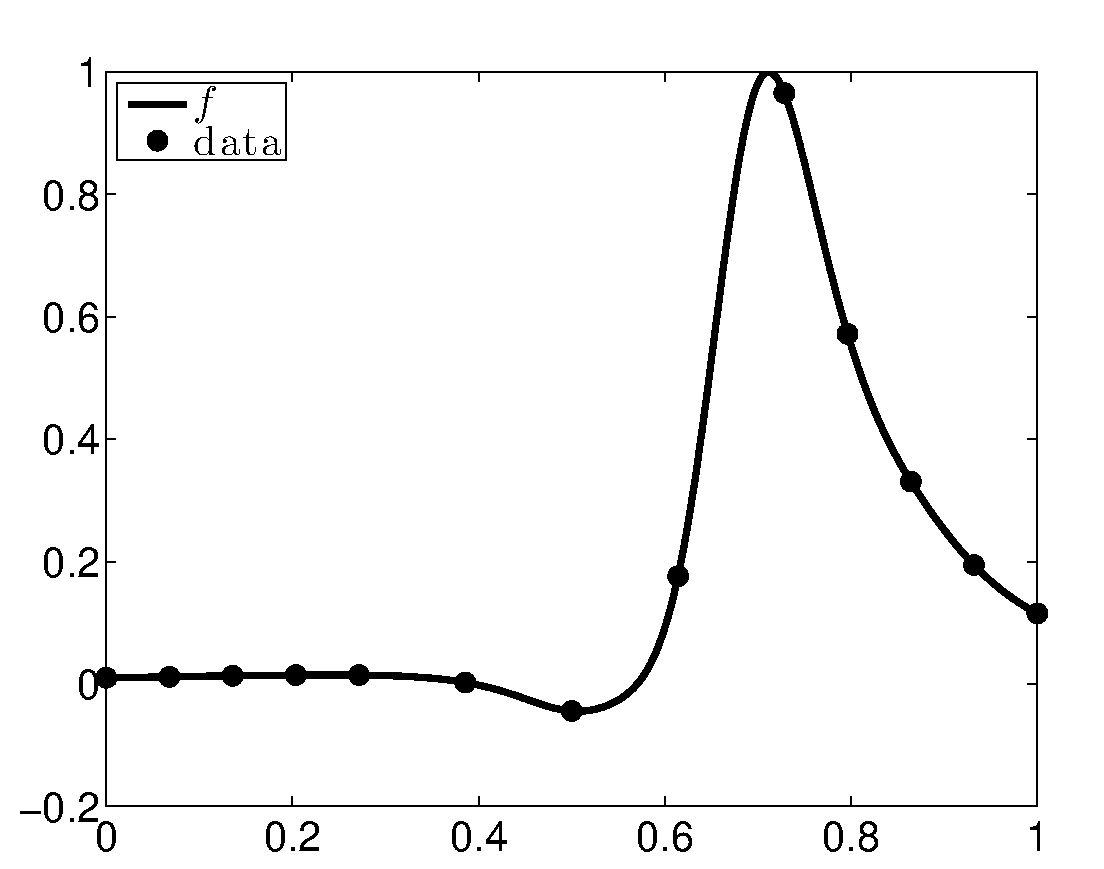
\includegraphics[width=8cm]{foolbwquadexample.eps}
\caption{Integrand designed to fool MATLAB's {\tt quad} along with the data used by {\tt quad}. \label{fig:foolquad}}
\end{figure}

While Lyness's argument is correct, it does not apply to the algorithms proposed in this article because their stopping criteria are not based on  $A_{n_{i}}(f)-A_{n_{i-1}}(f)$.  Algorithm \ref{multistageintegalgo} presented in Section \ref{integsec}, always succeeds for ``reasonable'' integrands because such integrands lie in the cone $\cc_{\tau}$.  The analogous statement is true for function approximation Algorithm \ref{multistageapproalgo}, as well as for the general Algorithms \ref{twostagedetalgo} and \ref{multistagealgo}.  All of these algorithms succeed for reasonable input functions.  

Lyness's warning in \cite{Lyn83} should not be interpreted as an objection to automatic algorithms.  It is a valid objection to stopping criteria that are based on the value of a single functional, in this case, $A_{n_{i}}-A_{n_{i-1}}$.  What Lyness clearly demonstrates is that one may easily make a functional vanish even though the error of the algorithm is significant.

\subsection{No Advantage in Adaption}

Although there are some positive results on adaption in \cite{Nov96a,PlaWas05a,PlaEtal08a}, there are also sweeping, rigorous results from information based complexity theory stating that adaptive algorithms have no significant advantage over non-adaptive algorithms (e.g., see \citep[Chapter 4, Theorem 5.2.1]{TraWasWoz88} and \cite{Nov96a}). The automatic algorithms presented here do adaptively determine the total number of samples required based on the function data collected.  The reason that adaption can help in this context is that the cone of input functions, $\cc_{\tau}$, is not a convex set.  This violates one of the assumptions required to prove the negative results that adaption does not help.

To see why $\cc_{\tau}$ is not convex, let $f_{\text{in}}$ and $f_{\text{out}}$ be functions in $\cf$ with nonzero $\tcf$-semi-norms, where $f_{\text{in}}$  lies in the interior of this cone, and $f_{\text{out}}$ lies outside the cone.  This means that 
\[
\frac{\Fnorm{f_{\text{in}}}} {\Ftnorm{f_{\text{in}}}} = \tau_{\text{in}} < \tau < \tau_{\text{out}} =  \frac{\Fnorm{f_{\text{out}}}} {\Ftnorm{f_{\text{out}}}}.
\]
Next define two functions in terms of $f_{\text{in}}$ and $f_{\text{out}}$ as follows:
\[
f_{\pm} = (\tau-\tau_{\text{in}}) \Ftnorm{f_{\text{in}}} f_{\text{out}}  \pm (\tau + \tau_{\text{out}}) \Ftnorm{f_{\text{out}}} f_{\text{in}},
\]
These functions must lie inside  $\cc_{\tau}$ because
\begin{align*}
\frac{\Fnorm{f_{\pm}}} {\Ftnorm{f_{\pm}}} 
&= \frac{\Bigl \lVert (\tau-\tau_{\text{in}}) \Ftnorm{f_{\text{in}}} f_{\text{out}}  \pm (\tau + \tau_{\text{out}}) \Ftnorm{f_{\text{out}}} f_{\text{in}}\Bigr \rVert_{\cf}}
{\Bigl \lVert (\tau-\tau_{\text{in}}) \Ftnorm{f_{\text{in}}} f_{\text{out}}  \pm (\tau + \tau_{\text{out}}) \Ftnorm{f_{\text{out}}} f_{\text{in}}\Bigr \rVert_{\tcf}}\\
& \le 
\frac{(\tau-\tau_{\text{in}}) \Ftnorm{f_{\text{in}}} \Fnorm{f_{\text{out}}}  + (\tau + \tau_{\text{out}}) \Ftnorm{f_{\text{out}}} \Fnorm{f_{\text{in}}}}
{-(\tau-\tau_{\text{in}}) \Ftnorm{f_{\text{in}}} \Ftnorm{f_{\text{out}}}  + (\tau + \tau_{\text{out}}) \Ftnorm{f_{\text{out}}} \Ftnorm{f_{\text{in}}}}\\
& =
\frac{(\tau-\tau_{\text{in}})\tau_{\text{out}}  + (\tau + \tau_{\text{out}}) \tau_{\text{in}} } {-(\tau-\tau_{\text{in}}) + (\tau + \tau_{\text{out}})}
=
\frac{\tau (\tau_{\text{out}} +\tau_{\text{in}}) } {\tau_{\text{out}} + \tau_{\text{in}}} =  \tau.
\end{align*}
On the other hand, the average of $f_{\pm}$, which is also a convex combination is 
\[
\frac{1}{2} f_- + \frac{1}{2} f_+ = (\tau-\tau_{\text{in}}) \Ftnorm{f_{\text{in}}} f_{\text{out}}.
\]
Since $\tau > \tau_{\text{in}}$, this is a nonzero multiple of $f_{\text{out}}$, and it lies outside $\cc_{\tau}$.  Thus, this cone is not a convex set.


\section{Discussion and Further Work} \label{furthersec}

When we consider the landscape of numerical algorithms, it is clear that relatively simple problems have well-developed automatic algorithms that we use without questioning their reliability.  For example, the MATLAB \cite{MAT7.12} algorithms
\[
{\tt cos, sin, exp, log, airy, besselj, gamma, gammainc, ellipj, erf,} \text{ and } {\tt  erfinv}
\] 
all automatically use the correct number of terms in a suitable expansion needed to provide the corresponding function value with $15$ significant digit accuracy. The only exceptions are cases of unavoidable round-off error, e.g., 
\[
{\tt cos(1e47*pi)= -5.432862626006405e-01},
\]
whereas the correct answer is {\tt 1}.  

We believe that more complex problems, whose inputs are functions, also deserve to have automatic algorithms with guarantees of their success.  Users ought to be able to integrate functions, approximate functions, optimize functions, etc., without needing to manually tune the sample size.  Here we have shown how this might be done in general, as well as specifically for two case studies.  We hope that this will inspire further research in this direction.



The results presented here suggest a number of other interesting open problems.  Here is a summary.

\begin{itemize}

\item Here we consider an absolute error tolerance.  This analysis should be extended to relative error, which is work in progress.  

\item The univariate integration and function approximation algorithms in Sections \ref{integsec} and \ref{approxsec} have low order convergence.  Guaranteed automatic algorithms with \emph{higher order convergence rates} for smoother input functions are needed.  These might be based on higher degree piecewise polynomial approximations.

\item There are other types of problems, e.g., differential equations and nonlinear optimization, which fit the general framework presented here.  These problems also have automatic algorithms, but without guarantees.  It would be helpful to develop guaranteed automatic algorithms in these other areas.

\item The algorithms developed here are \emph{globally adaptive}, in the sense that the function data determines the sample size, but not the kinds of data collected or the locations of the sample points, which depend only on the sample size.  Some existing automatic algorithms are \emph{locally adaptive} in that they collect more data in regions of special interest, say where the function has a spike.  Such algorithms need guarantees like the ones that are provided here for globally adaptive algorithms.  The appropriate kinds of spaces $\tcf$ and $\cf$, and their semi-norms, need to be identified for locally adaptive algorithms.

\item For some numerical problems the error bound of the non-adaptive algorithm involves a $\tcf$- or $\cf$-semi-norm that is very hard to approximate because of its complexity.  An example is multivariate quadrature using quasi-Monte Carlo algorithms, where the error depends on the \emph{variation} of the integrand.  The definition of the variation depends on the definition of $\tcf$ or $\cf$, but it is essentially some semi-norm of a mixed partial derivative of the integrand.  To obtain guaranteed automatic algorithms one must either find an efficient way to approximate the variation of the function or find other suitable conservative estimates for the error that can be reliably obtained from the function data.  

\item This article considers only the worst case error of deterministic algorithms.  There are many random algorithms, and they must be analyzed by somewhat different methods.  A guaranteed Monte Carlo algorithm for estimating the mean of a random variable, which includes multivariate integration as a special case, has been proposed in \cite{HicEtal14a}.

\end{itemize}

\section{Acknowledgements}  The authors are grateful for discussions with a number of colleagues. This research is supported in part by grant NSF-DMS-1115392.

\section*{References}
\bibliographystyle{model1b-num-names.bst}
%\bibliographystyle{elsarticle-num-names}
\bibliography{FJH22,FJHown22}
\end{document}

